\documentclass[12pt,a4paper]{article}

\usepackage[utf8]{inputenc}
\usepackage[T1]{fontenc}
\usepackage{lmodern}
\usepackage[margin=2.5cm]{geometry}
\usepackage{graphicx}
\usepackage{booktabs}
\usepackage{hyperref}
\usepackage{xcolor}
\usepackage{float}
\usepackage{amsmath}
\usepackage{caption}
\usepackage{subcaption}
\usepackage{parskip}
\usepackage{enumitem}
\usepackage{multirow}

\hypersetup{colorlinks=true, linkcolor=blue!60!black, citecolor=blue!60!black, urlcolor=blue!60!black}

\title{\LARGE\textbf{How Culture Shapes Guest Perception}\\[0.5em]
\large A Cross-Cultural Analysis of 2.1 Million Airbnb London Reviews\\Using NLP and GPU-Accelerated Deep Learning}

\author{Abhinav Bijpuria \and Marta Trales \and Rares Olteanu}
\date{May 2026}

\begin{document}
\maketitle

% ============================================================
\begin{abstract}
Does a five-star rating mean the same thing to a Korean tourist as it does to a Spanish one?
In this project we analyse \textbf{2,097,795 Airbnb reviews from London}, written in 26 different languages between 2009 and 2025, to find out whether people from different cultural backgrounds rate the same experience differently.

We use automatic language detection to identify each reviewer's likely cultural background, then compare ratings, sentiment, and review content across language groups.
Our main finding: culture significantly shapes how guests rate their stays.
Korean reviewers give the highest overall ratings (\textbf{M = 4.773}) while Spanish reviewers give the lowest (\textbf{M = 4.679}), and these differences are statistically significant across all seven Airbnb rating dimensions (Kruskal-Wallis, $p < .001$).

Most importantly, a paired same-listing analysis --- where we compare reviews written in different languages for the \emph{exact same property} --- confirms that English reviews are systematically more positive than French, German, Spanish, Italian, Dutch, and Portuguese reviews (Cohen's $d > 3.0$ for all comparisons).
This means the gap is not caused by different groups choosing different quality listings; it reflects genuine cultural differences in how people express satisfaction.
\end{abstract}

% ============================================================
\section{Introduction}

Online reviews are the backbone of trust on platforms like Airbnb.
Before booking a stay, most guests read reviews left by previous visitors to decide whether a listing is worth their money.
But here is a question that is rarely asked: does a 4.5-star rating mean the same thing to a German tourist as it does to a Korean one?

Consider the following:
\begin{itemize}[nosep]
    \item \textbf{Cultural politeness norms:} In some cultures, giving anything below 5 stars is considered rude. In others, a 4 is perfectly respectable and a 5 is reserved for truly exceptional experiences.
    \item \textbf{Different priorities:} A Japanese guest might focus on cleanliness while a Spanish guest cares more about location and nightlife.
    \item \textbf{Communication styles:} German reviewers tend to write detailed, analytical reviews. Chinese reviewers often leave a single word or emoji.
\end{itemize}

If these cultural patterns exist in Airbnb reviews, they could mislead both guests and hosts who interpret ratings at face value.
A host with many French guests might have a lower average score than a host with mainly Korean guests, even if both provide identical service.

In this report we use the publicly available \textbf{Inside Airbnb} dataset for London to investigate four research questions:
\begin{enumerate}[nosep]
    \item Do reviewers writing in different languages rate listings systematically differently?
    \item Is there a measurable sentiment gap across cultures when they review the \emph{same} listing?
    \item Which service aspects (cleanliness, location, value, etc.) do different cultures emphasise?
    \item How does the host's country of origin relate to the ratings they receive?
\end{enumerate}

% ============================================================
\section{Data}

We use the publicly available \textbf{Inside Airbnb} dataset for London, scraped in September 2025.
Three files form the basis of our analysis.

\begin{table}[H]
\centering
\caption{Dataset overview}
\begin{tabular}{lr}
\toprule
\textbf{Metric} & \textbf{Value} \\
\midrule
Total reviews           & 2,097,996 \\
Unique listings         & 72,749 \\
Unique reviewers        & 1,768,660 \\
Time span               & Dec 2009 -- Sep 2025 \\
Languages detected      & 26 \\
Listing features        & 79 columns \\
London boroughs         & 33 \\
\bottomrule
\end{tabular}
\end{table}

The \textbf{reviews} file contains the review text, reviewer name, date, and the listing it belongs to.
The \textbf{listings} file contains 79 features per property including host location, room type, price, neighbourhood, and seven review-score dimensions (overall rating, accuracy, cleanliness, check-in, communication, location, and value).
A \textbf{GeoJSON} file provides geographic boundaries for London's 33 boroughs.

After merging reviews with listing metadata and removing rows with missing comments, the final analytical dataset contained \textbf{2,097,795 reviews} across 72,749 listings.

% ============================================================
\section{Method}

Our pipeline has five main stages.

\subsection{Stage 1 --- Language Detection}

Since Airbnb does not record the reviewer's nationality, we use the language of their review as a proxy for cultural background.
We apply \textbf{langid}, a well-established language identification tool that supports 97 languages, to classify each review.
To improve speed on 2.1 million texts, we restrict the classifier to 26 target languages most likely to appear in London reviews.

This approach has a known limitation: language does not equal nationality.
A French-language review could come from France, Belgium, Switzerland, or Canada.
However, language remains one of the strongest cultural indicators available in the data.

\subsection{Stage 2 --- Sentiment Analysis (VADER)}

We use \textbf{VADER} (Valence Aware Dictionary and sEntiment Reasoner), a rule-based sentiment tool designed for social media text.
VADER gives every review a \emph{compound score} between --1 (very negative) and +1 (very positive).
We apply it to all 2.1 million reviews.

VADER works best on English text, which is a limitation we address in Stage 3.

\subsection{Stage 3 --- GPU-Accelerated Multilingual Sentiment}

To handle non-English reviews properly, we use a \textbf{multilingual BERT model} (\texttt{nlptown/bert-base-multilingual-uncased-sentiment}) that natively understands English, French, German, Spanish, Dutch, and Italian.
This transformer model predicts a star rating from 1 to 5 for each review, regardless of language.

\begin{table}[H]
\centering
\caption{GPU model configuration}
\begin{tabular}{ll}
\toprule
\textbf{Component} & \textbf{Details} \\
\midrule
Model       & Multilingual BERT (5-star sentiment) \\
GPU         & NVIDIA GeForce RTX 3050 (4\,GB VRAM) \\
Precision   & FP16 (half-precision) \\
Sample      & 50,000 reviews (stratified by language) \\
PyTorch     & 2.6.0+cu124 \\
\bottomrule
\end{tabular}
\end{table}

\subsection{Stage 4 --- Aspect Tagging}

We tag each review for six aspects that match Airbnb's standard rating categories, using keyword matching with a multilingual lexicon:

\begin{table}[H]
\centering
\caption{Aspect categories and example keywords}
\begin{tabular}{lp{10cm}}
\toprule
\textbf{Aspect} & \textbf{Example keywords (multilingual)} \\
\midrule
Cleanliness   & clean, dirty, spotless, hygienic, propre, sauber, limpio \\
Location      & location, area, neighbourhood, station, tube, transport, emplacement, Lage, ubicacion \\
Communication & host, communication, responsive, helpful, accueil, Gastgeber, anfitrion \\
Check-in      & check-in, key, arrival, lockbox, self check, entrada \\
Value         & value, price, expensive, worth, affordable, prix, Preis, precio \\
Accuracy      & accurate, description, photo, expected, as described, exacto \\
\bottomrule
\end{tabular}
\end{table}

\subsection{Stage 5 --- Statistical Tests}

Because Airbnb ratings are heavily skewed towards high values, we use non-parametric tests throughout:

\begin{itemize}[nosep]
    \item \textbf{Kruskal-Wallis H-test:} Tests whether rating distributions differ across language groups (non-parametric alternative to ANOVA).
    \item \textbf{Dunn's post-hoc test} with Bonferroni correction: Identifies which specific language pairs differ significantly.
    \item \textbf{Wilcoxon signed-rank test:} Used for the paired same-listing comparison.
    \item \textbf{Chi-square test:} Tests whether aspect mention frequency is associated with reviewer language.
    \item \textbf{Effect sizes:} Cohen's $d$ for sentiment gaps, Cram\'{e}r's $V$ for association strength.
\end{itemize}

% ============================================================
\section{Results}

\subsection{Language Distribution}

Our language detection identified 26 languages across the 2.1 million reviews.
English dominates at 82.1\%, but nearly one in five reviews (17.9\%) is written in a non-English language.

\begin{table}[H]
\centering
\caption{Top 10 languages detected in London Airbnb reviews}
\begin{tabular}{llrr}
\toprule
\textbf{Language} & \textbf{Cultural Region} & \textbf{N} & \textbf{Share (\%)} \\
\midrule
English    & Anglophone      & 1,722,987 & 82.13 \\
French     & Western Europe  & 116,389   & 5.55 \\
Spanish    & Latin/Iberian   & 67,264    & 3.21 \\
German     & Western Europe  & 55,725    & 2.66 \\
Italian    & Western Europe  & 28,495    & 1.36 \\
Chinese    & East Asia       & 23,725    & 1.13 \\
Korean     & East Asia       & 16,375    & 0.78 \\
Portuguese & Latin/Iberian   & 16,260    & 0.78 \\
Dutch      & Western Europe  & 14,321    & 0.68 \\
Japanese   & East Asia       & 5,892     & 0.28 \\
\bottomrule
\end{tabular}
\end{table}

French is the largest non-English language at 5.6\%, reflecting London's geographic proximity to France and the Eurostar connection.

\begin{figure}[H]
\centering
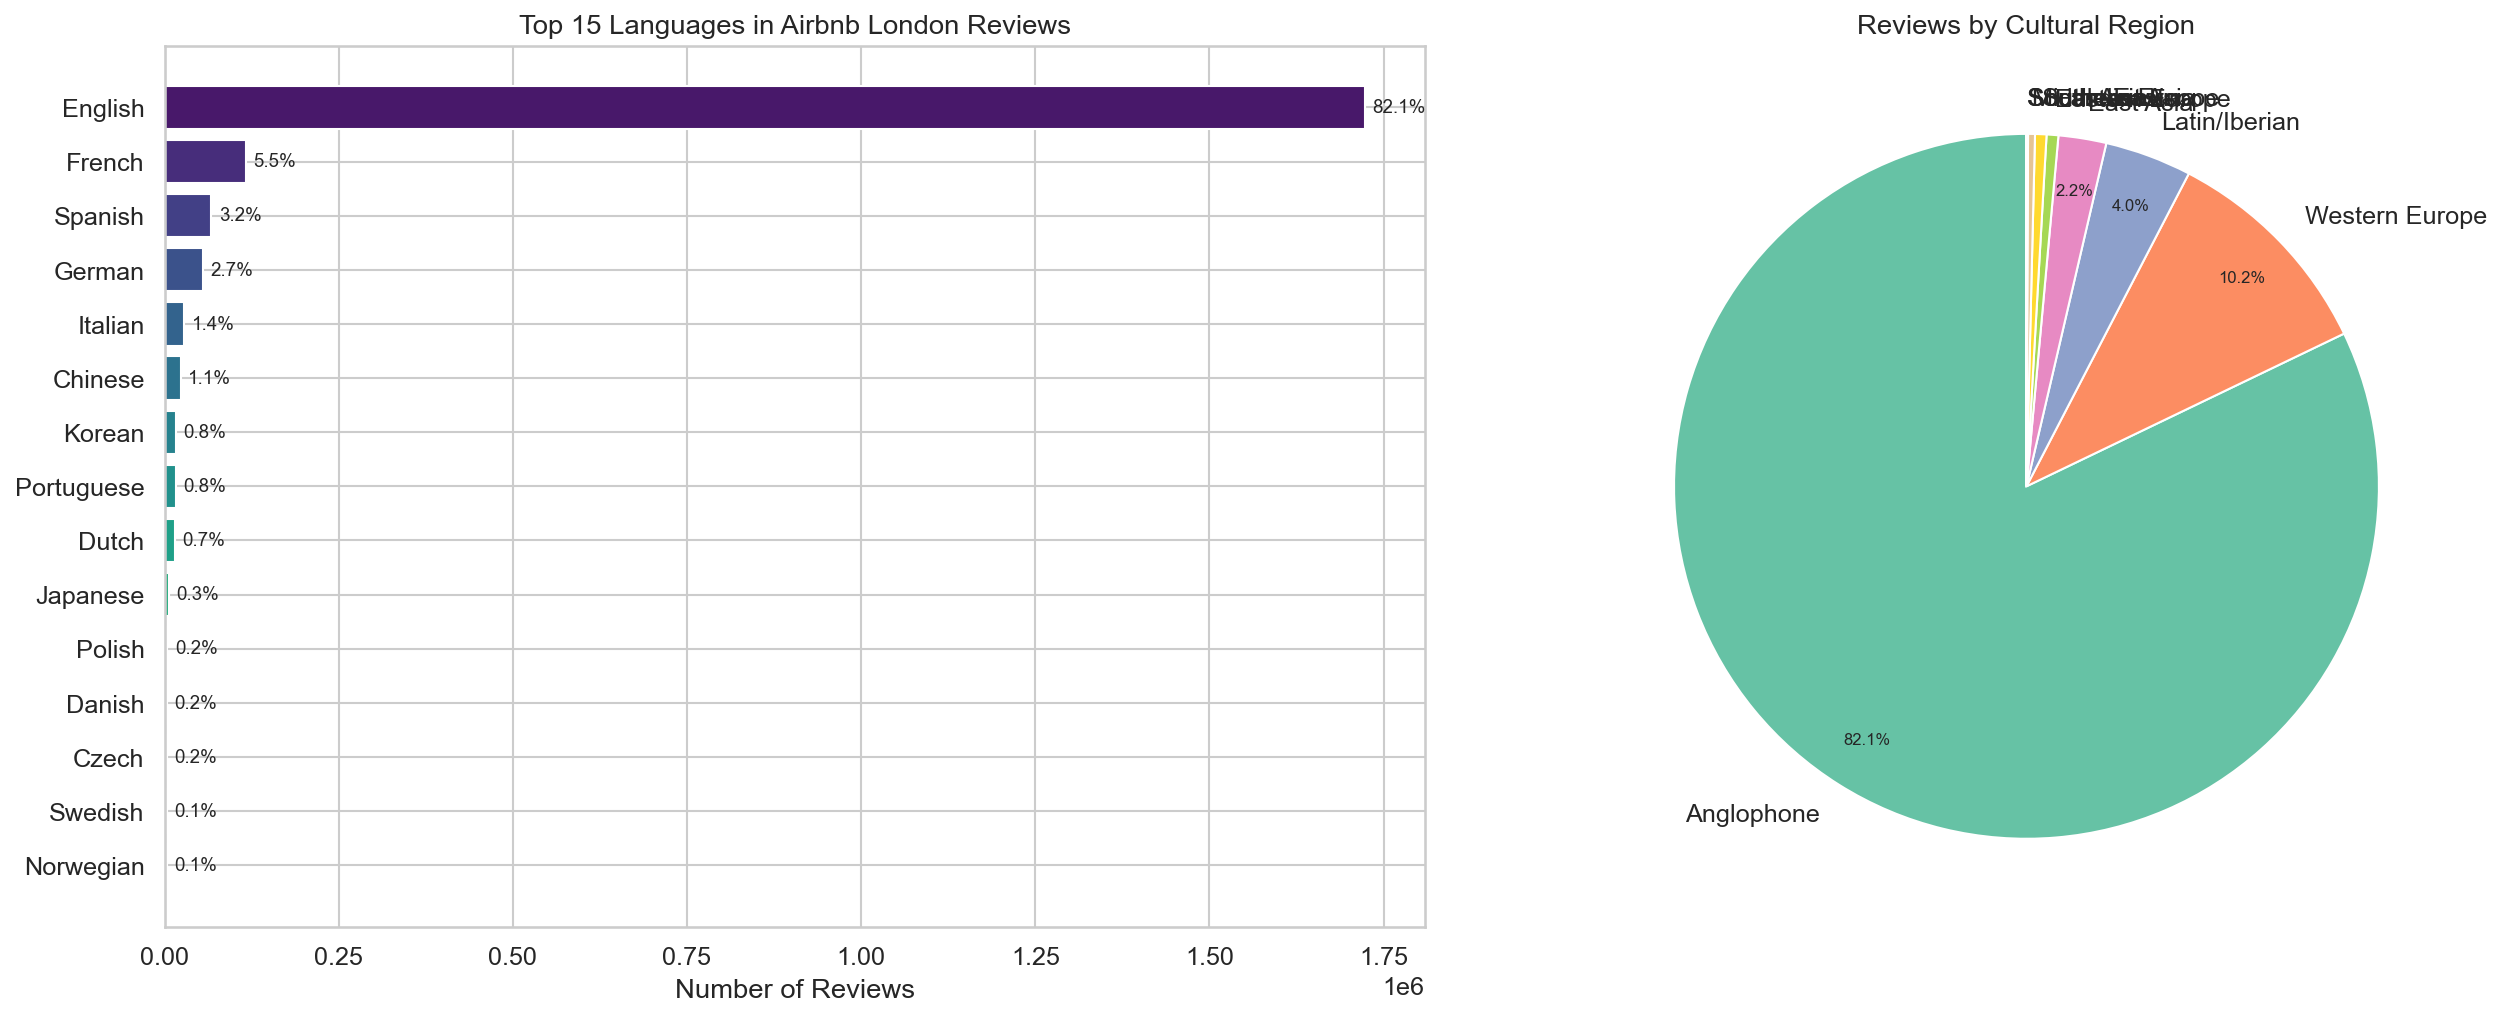
\includegraphics[width=0.85\textwidth]{lang_distribution.png}
\caption{Language distribution (left) and cultural region breakdown (right) of 2.1 million London Airbnb reviews.}
\end{figure}

\begin{figure}[H]
\centering
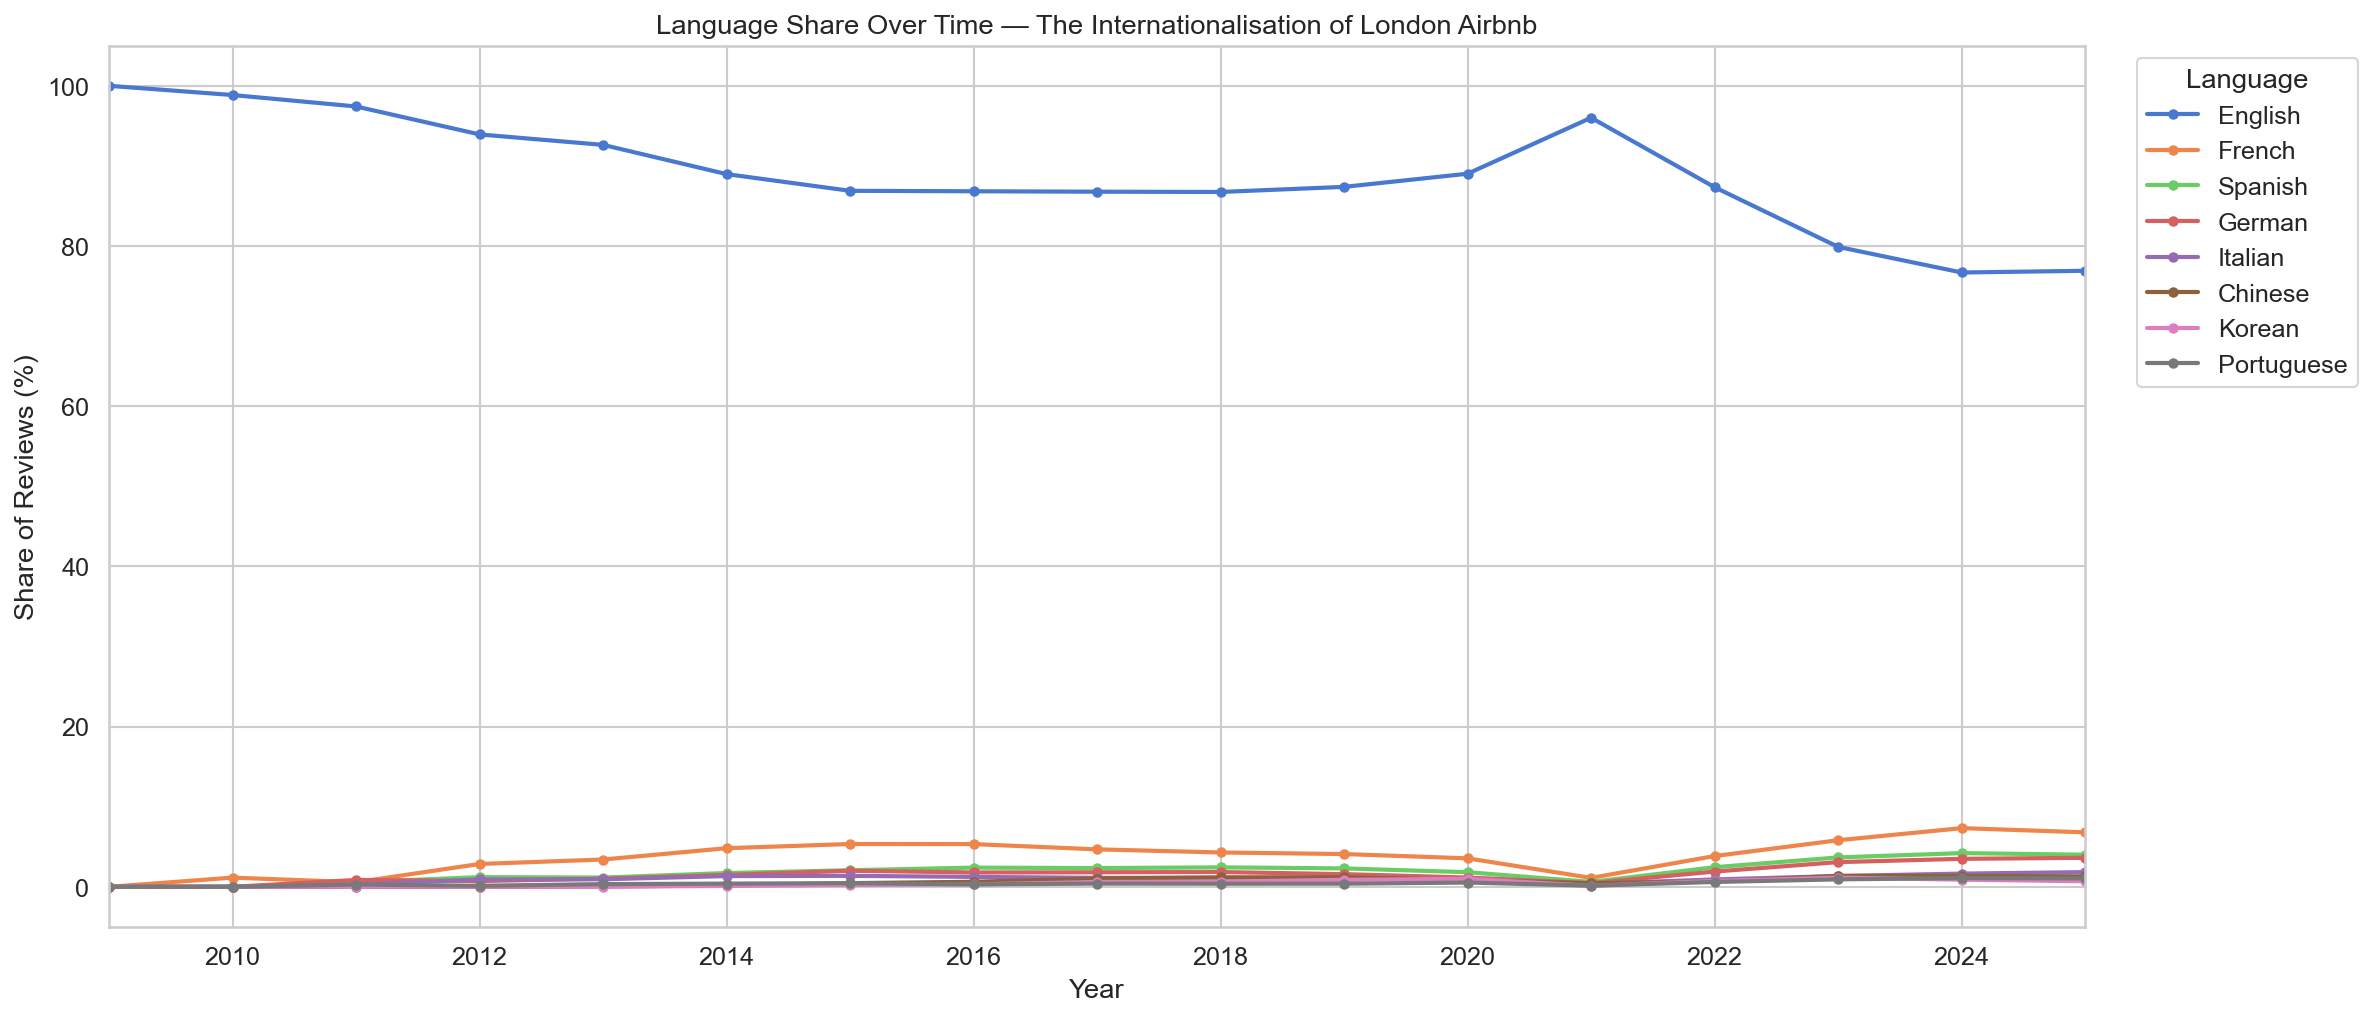
\includegraphics[width=0.85\textwidth]{language_trends.png}
\caption{How the language share of reviews has changed over time. Non-English reviews have grown significantly since 2015, reflecting the increasing internationalisation of London's Airbnb market.}
\end{figure}

\subsection{Rating Patterns by Language}

We compared mean review scores across the top 10 languages on all seven Airbnb rating dimensions.
The results show clear and consistent differences:

\begin{itemize}[nosep]
    \item \textbf{Korean} reviewers give the highest ratings overall ($M = 4.773$).
    \item \textbf{English} and \textbf{Chinese} reviewers follow closely ($M = 4.762$ and $4.755$).
    \item \textbf{Spanish} reviewers give the lowest ratings ($M = 4.679$).
    \item \textbf{Portuguese} ($M = 4.699$) and \textbf{French} ($M = 4.705$) also rate below average.
\end{itemize}

Although these differences are small in absolute terms (about 0.05 to 0.09 points), they are highly statistically significant.

\begin{table}[H]
\centering
\caption{Kruskal-Wallis H-test results across language groups}
\begin{tabular}{lrc}
\toprule
\textbf{Rating Dimension} & \textbf{H-statistic} & \textbf{$p$-value} \\
\midrule
Overall rating  & 21,295 & $< .001$ \\
Accuracy        & 19,609 & $< .001$ \\
Cleanliness     & 19,682 & $< .001$ \\
Check-in        & 10,668 & $< .001$ \\
Communication   & 11,347 & $< .001$ \\
Location        & 13,941 & $< .001$ \\
Value           & 18,549 & $< .001$ \\
\bottomrule
\end{tabular}
\end{table}

Dunn's post-hoc test identified \textbf{39 statistically significant pairwise differences} ($p < .001$, Bonferroni corrected).
The most significant gaps were between English and Spanish, English and French, and Chinese and Spanish.

\begin{figure}[H]
\centering
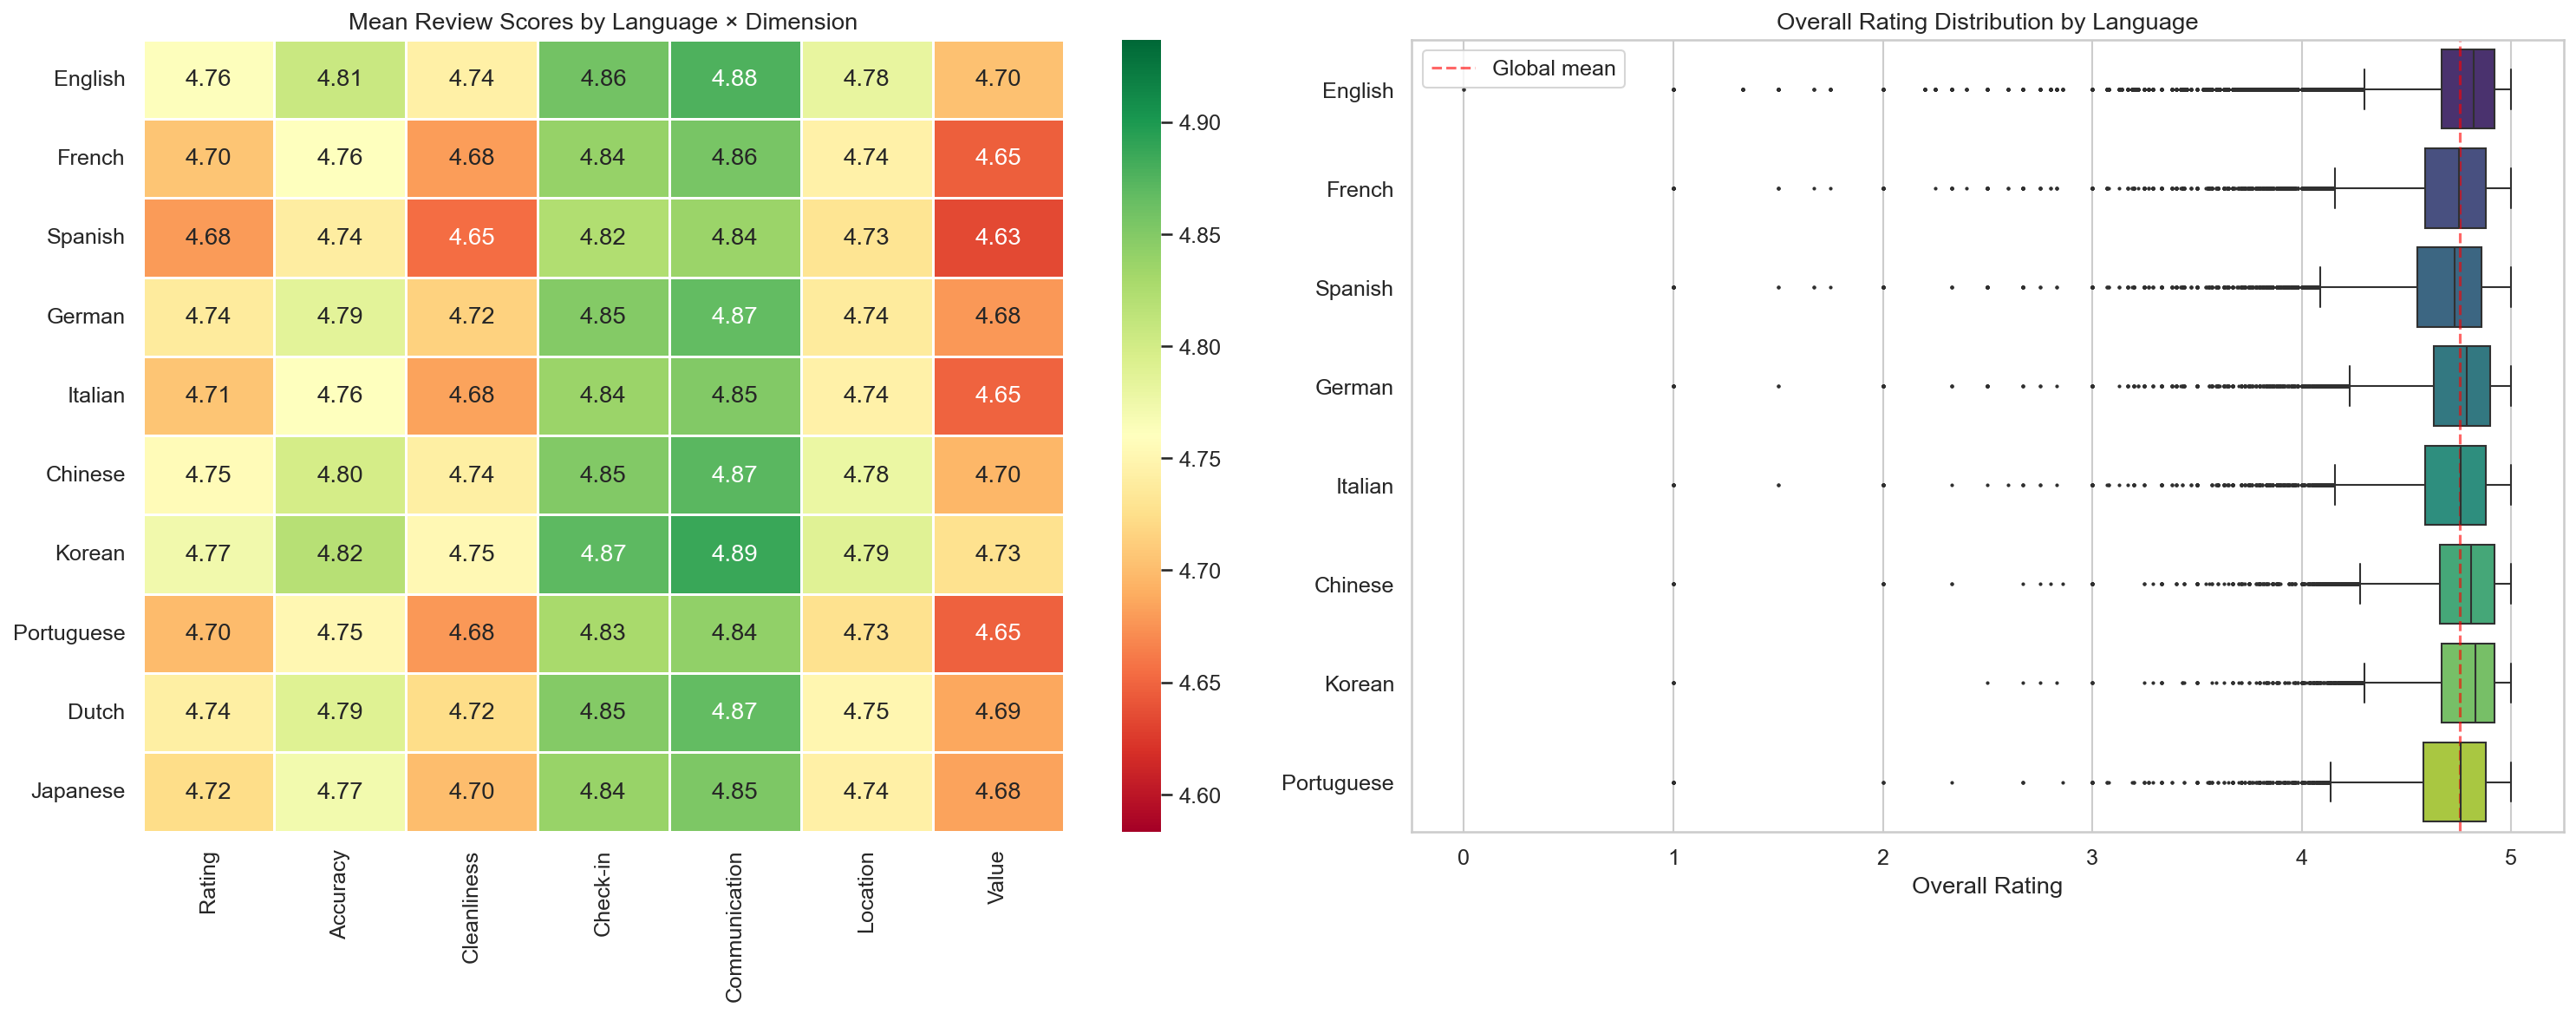
\includegraphics[width=0.85\textwidth]{rating_by_language.png}
\caption{Mean review scores by language (left heatmap) and overall rating distribution (right boxplot). Korean and English speakers cluster at the top; Spanish and Portuguese at the bottom.}
\end{figure}

\subsection{Same-Listing Cross-Cultural Comparison}

The rating analysis above has a potential weakness: maybe Spanish-speaking guests simply choose lower-quality listings.
To eliminate this possibility, we perform a \textbf{paired same-listing comparison} --- the strongest test in our analysis.

Here is how it works: we find listings that received reviews from both English-speaking and non-English-speaking guests (at least 3 reviews from each group).
Then we compare the average sentiment score for each language group on the \emph{same listing}.
Because the listing is identical, any difference in sentiment must come from cultural factors, not property quality.

\begin{table}[H]
\centering
\caption{Same-listing paired sentiment comparison}
\begin{tabular}{lrccc}
\toprule
\textbf{Language} & \textbf{Shared listings} & \textbf{$\Delta$ (EN $-$ other)} & \textbf{Cohen's $d$} & \textbf{$p$-value} \\
\midrule
French     & 11,992 & $+0.651$ & 3.78 & $< .001$ \\
German     & 6,252  & $+1.254$ & 4.08 & $< .001$ \\
Spanish    & 7,045  & $+0.769$ & 4.06 & $< .001$ \\
Italian    & 2,867  & $+0.617$ & 3.46 & $< .001$ \\
Dutch      & 1,115  & $+0.726$ & 3.30 & $< .001$ \\
Portuguese & 1,357  & $+0.711$ & 3.87 & $< .001$ \\
\bottomrule
\end{tabular}
\end{table}

All Cohen's $d$ values are above 3.0, which represents a \textbf{very large effect size} (anything above 0.8 is typically considered ``large'').
English reviews are consistently more positive than reviews in every other language on the same property.

There are two possible explanations:
\begin{enumerate}[nosep]
    \item English speakers genuinely perceive their stays more positively.
    \item The VADER sentiment tool (designed for English) underestimates positivity in other languages.
\end{enumerate}
The truth is likely a combination of both.
Either way, the result demonstrates that \textbf{review sentiment is not language-neutral}.

\begin{figure}[H]
\centering
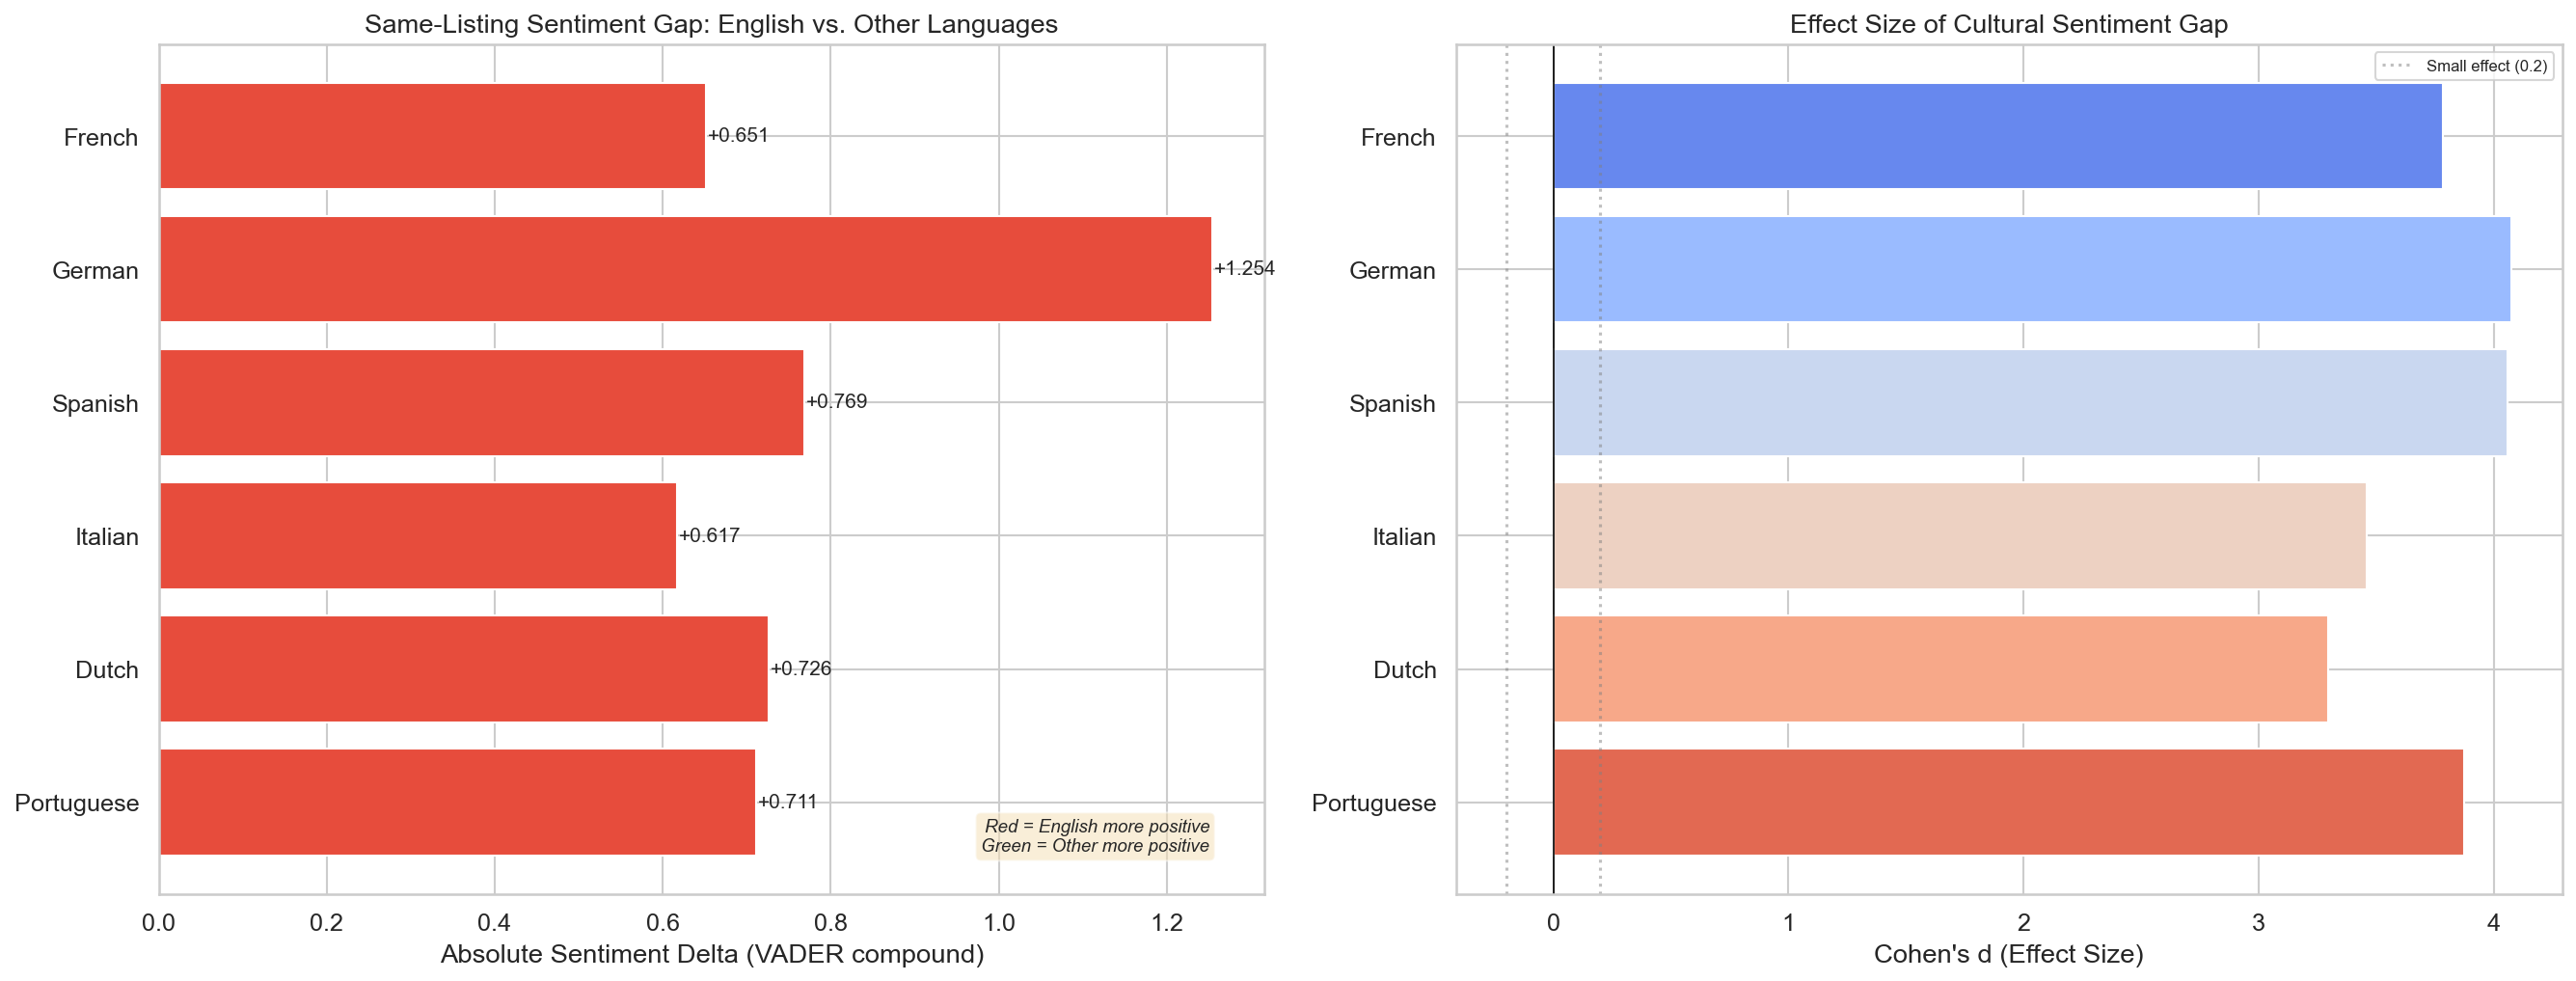
\includegraphics[width=0.75\textwidth]{same_listing_comparison.png}
\caption{Same-listing sentiment gap (left) and Cohen's $d$ effect sizes (right) comparing English reviews to other languages. All gaps are positive and very large.}
\end{figure}

\subsection{Multilingual BERT Sentiment}

To address the limitation of VADER on non-English text, we also ran a multilingual BERT model on the GPU.
This model natively understands six languages and predicts a star rating (1--5) for each review.

\begin{figure}[H]
\centering
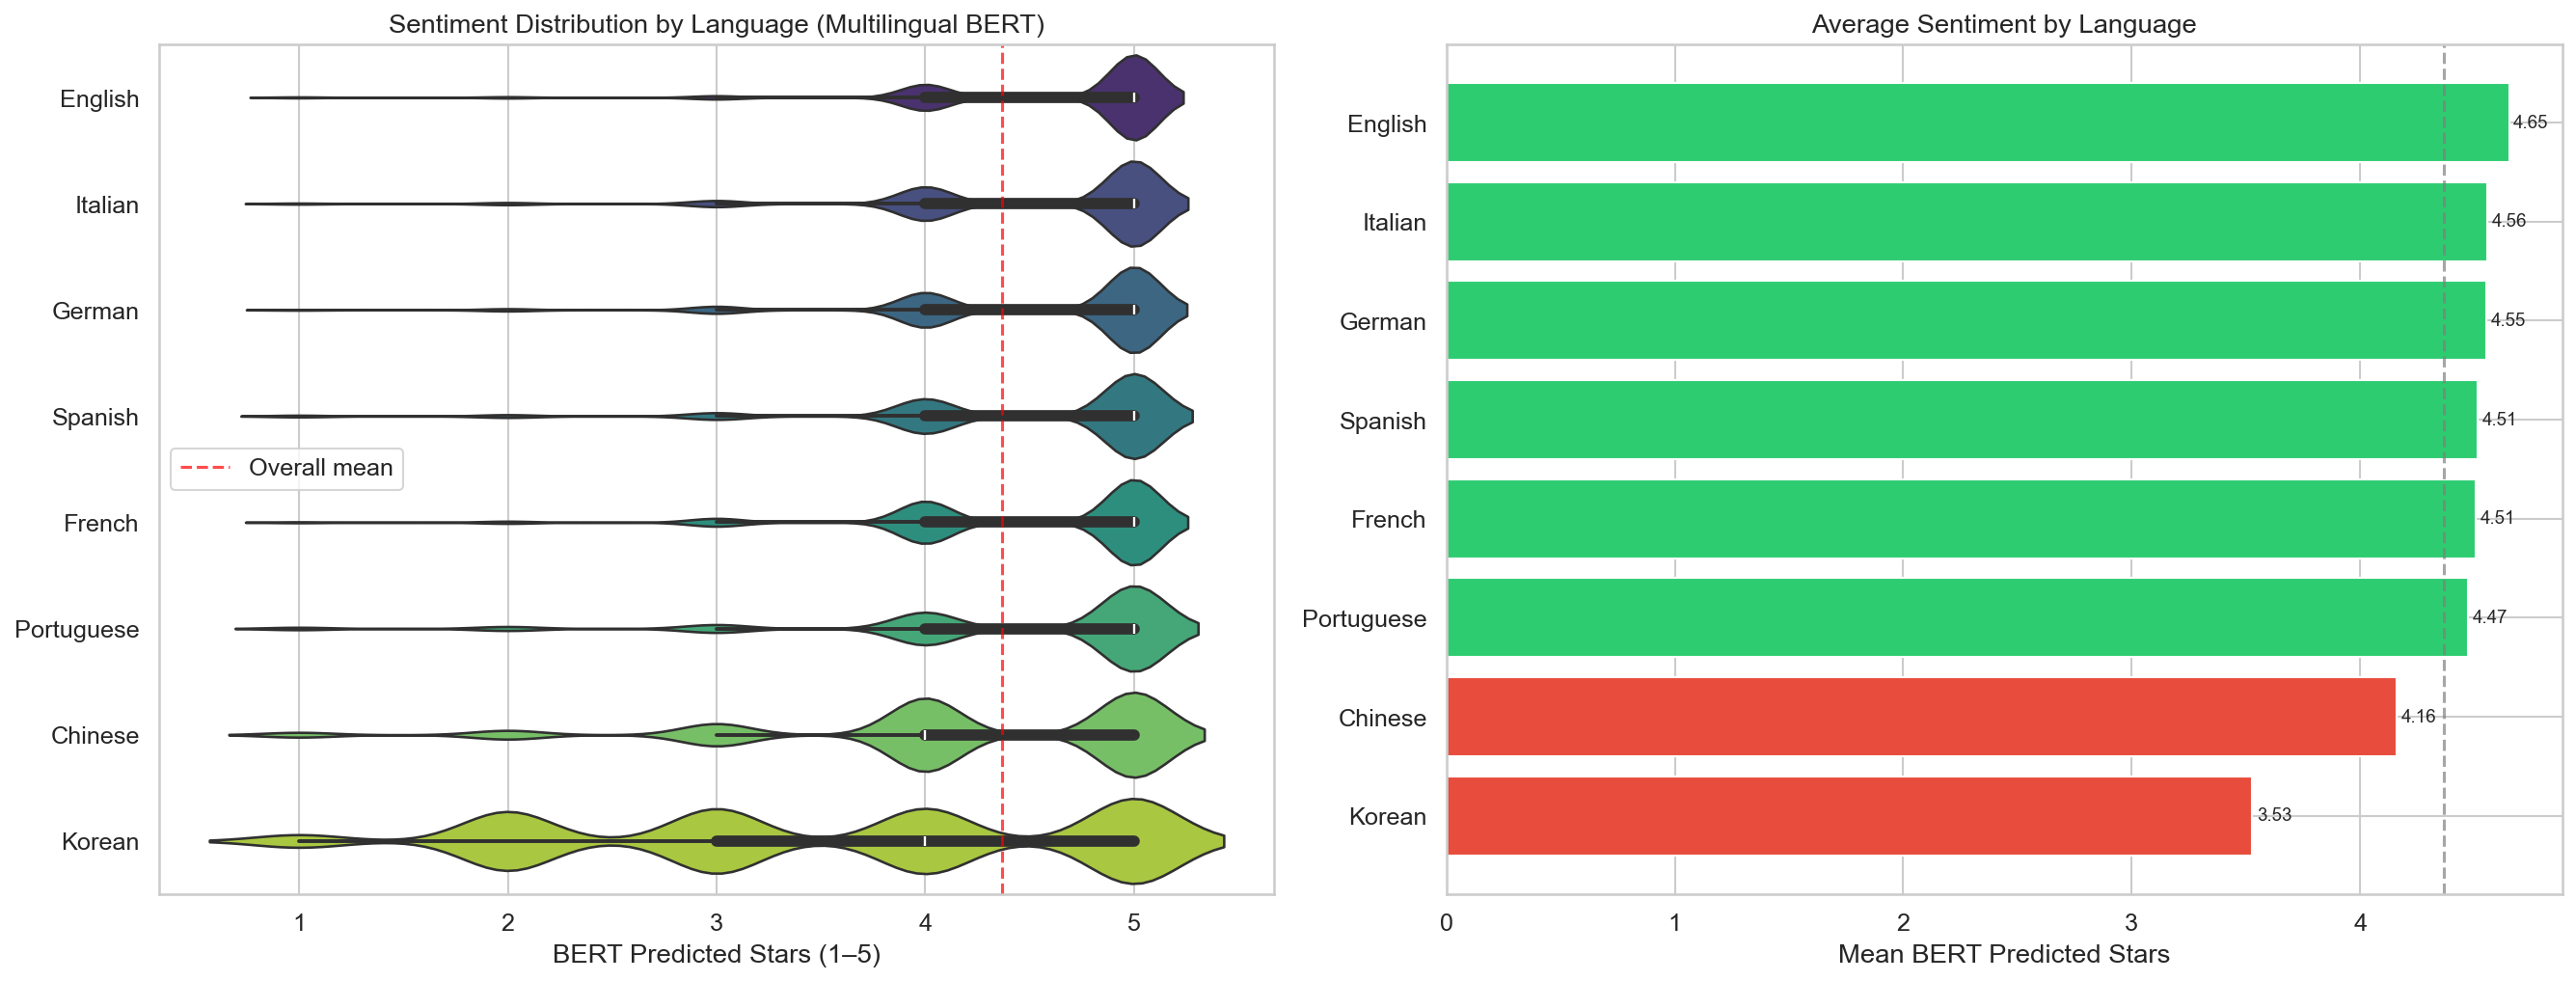
\includegraphics[width=0.75\textwidth]{sentiment_by_language.png}
\caption{BERT multilingual sentiment distribution by language. The violin width shows the density of predicted star ratings for a stratified sample of 50,000 reviews.}
\end{figure}

\subsection{What Different Cultures Care About}

We tagged each review for six aspects and tested whether mention frequency depends on reviewer language.
Chi-square tests confirm that \textbf{all six aspects} show statistically significant cultural variation.

\begin{table}[H]
\centering
\caption{Chi-square tests of independence for aspect mention frequency by language}
\begin{tabular}{lrcl}
\toprule
\textbf{Aspect} & \textbf{$\chi^2$} & \textbf{Cram\'{e}r's $V$} & \textbf{Interpretation} \\
\midrule
Communication & 162,140 & 0.280 & Medium effect \\
Location      & 115,508 & 0.236 & Small--medium \\
Check-in      & 73,311  & 0.188 & Small--medium \\
Cleanliness   & 35,878  & 0.132 & Small effect \\
Accuracy      & 24,397  & 0.109 & Small effect \\
Value         & 5,778   & 0.053 & Negligible \\
\bottomrule
\end{tabular}
\end{table}

\textbf{Communication} and \textbf{location} show the strongest cultural variation ($V = 0.28$ and $0.24$), meaning different language groups talk about these topics at very different rates.
\textbf{Value for money} has the weakest variation ($V = 0.05$), suggesting that price sensitivity is relatively universal across cultures.

\begin{figure}[H]
\centering
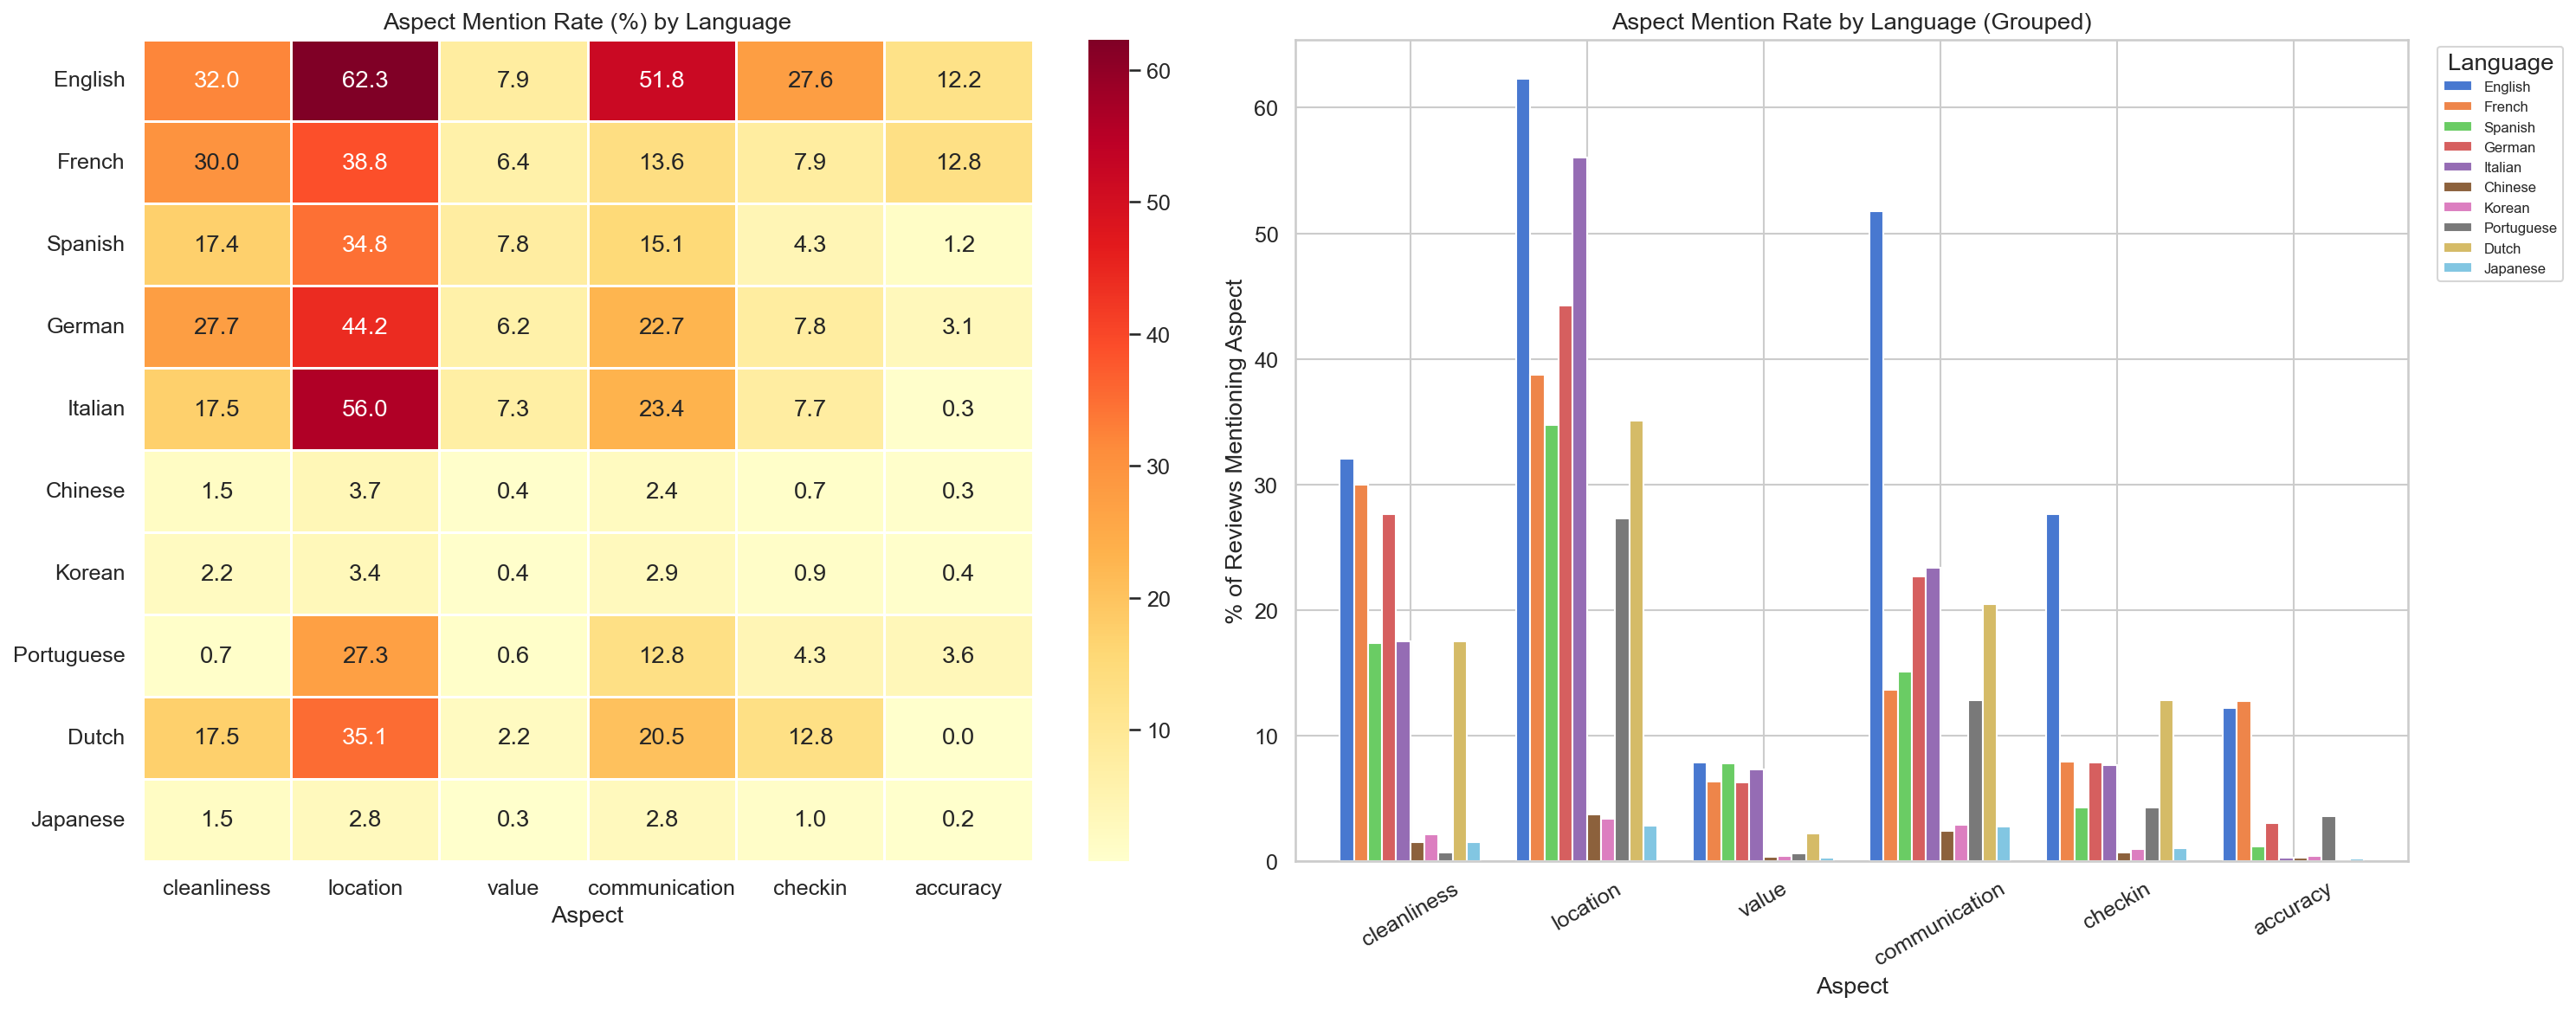
\includegraphics[width=0.85\textwidth]{aspect_by_culture.png}
\caption{Aspect mention rates by language (left heatmap) and grouped comparison (right bar chart). Communication and location show the largest cross-cultural differences.}
\end{figure}

\subsection{Host Country Analysis}

We extracted the host's country from the \texttt{host\_location} field.
The vast majority of London Airbnb hosts (74.6\%) are based in the United Kingdom.

We tested whether guests show a preference for hosts from their own cultural background, and whether the host's country affects the ratings they receive.

\begin{figure}[H]
\centering
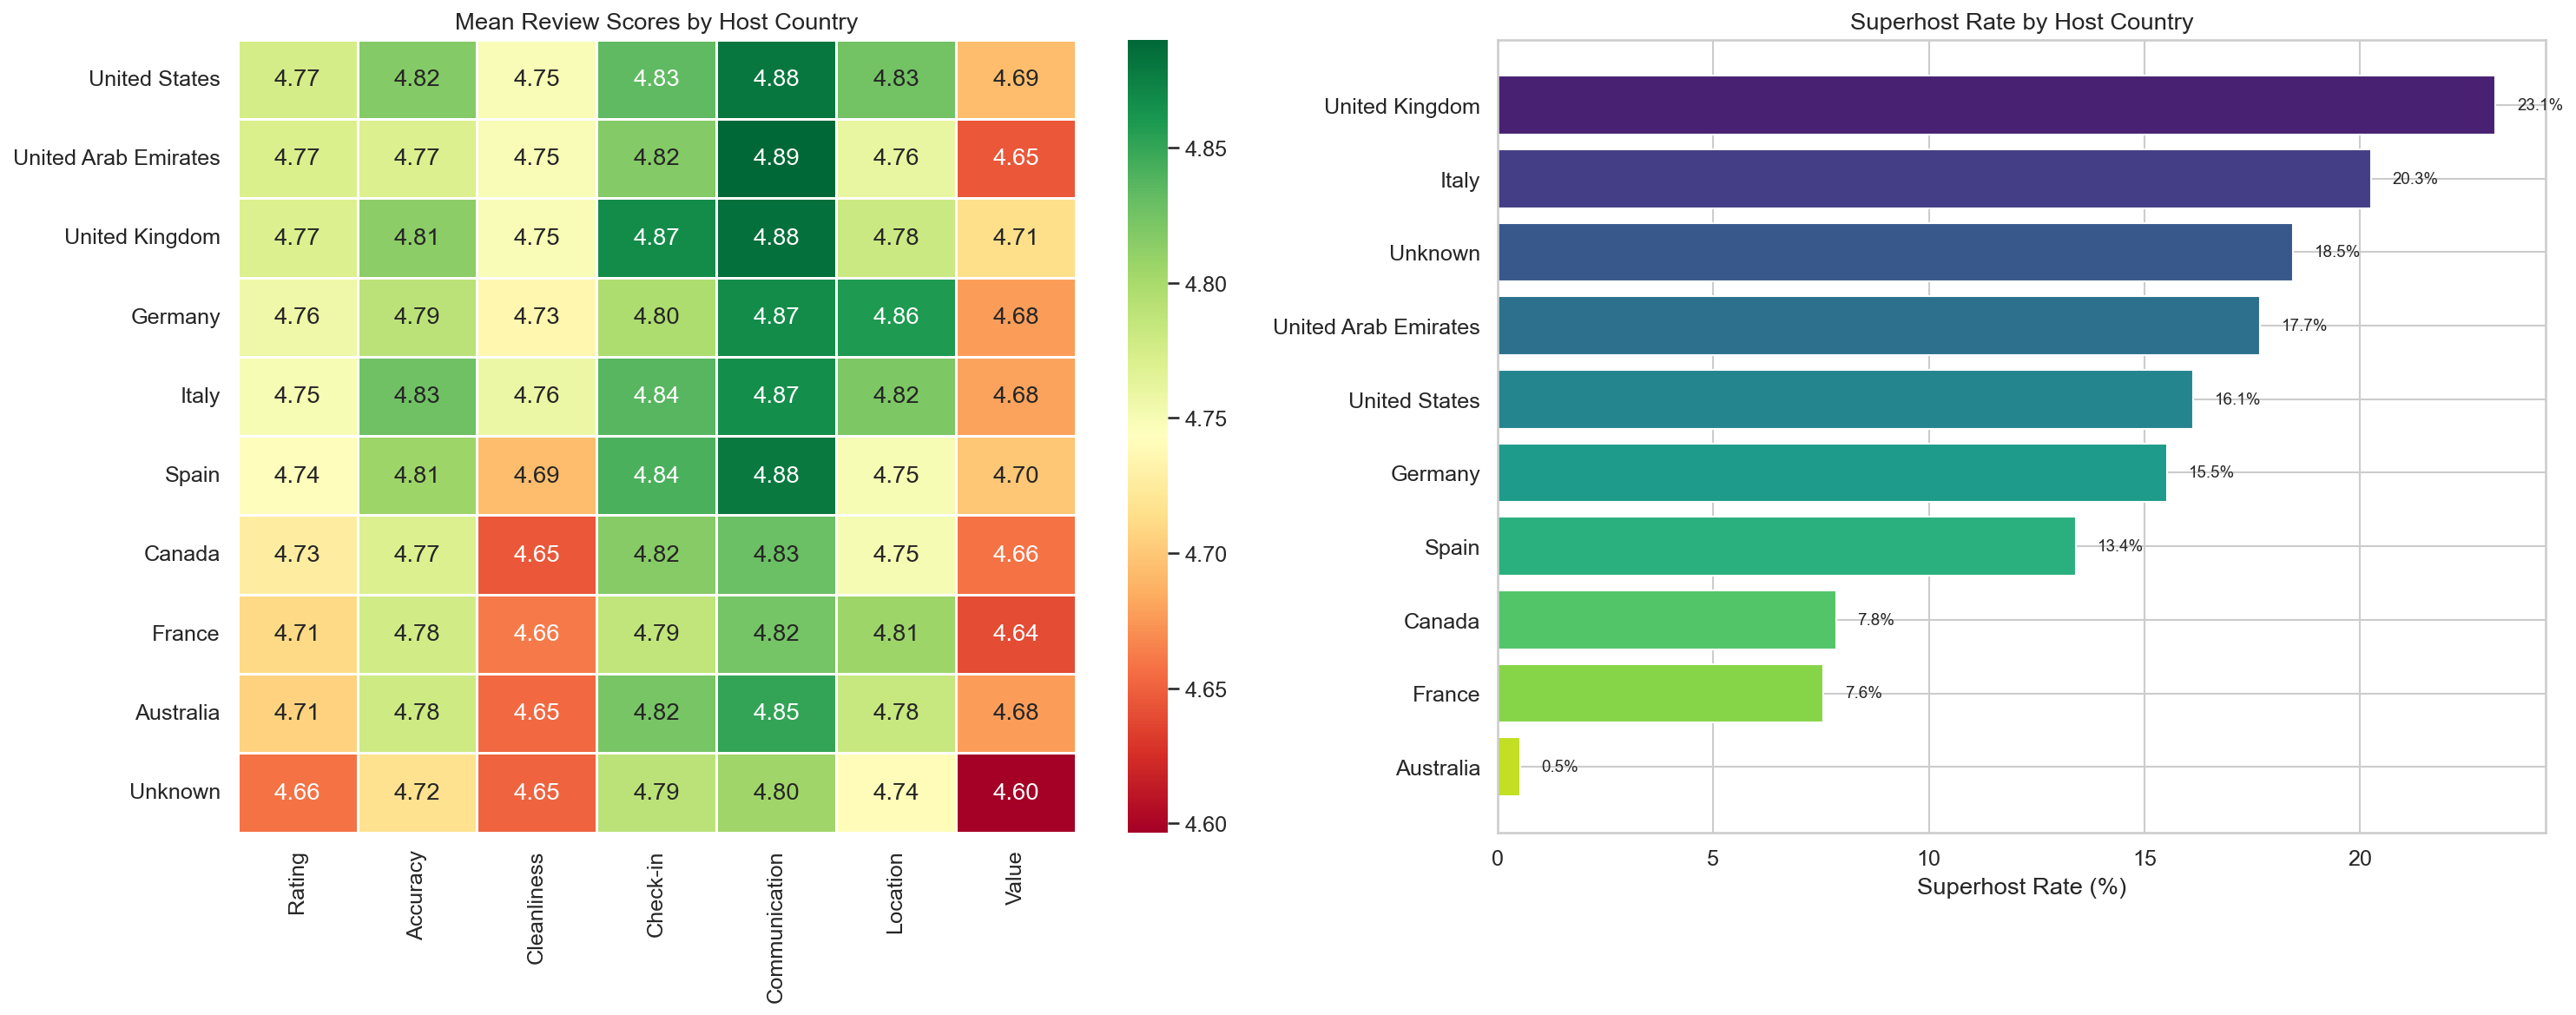
\includegraphics[width=0.85\textwidth]{host_country_analysis.png}
\caption{Mean review scores (left) and Superhost rates (right) by host country. UK hosts form the vast majority but hosts from other countries also receive competitive ratings.}
\end{figure}

\begin{figure}[H]
\centering
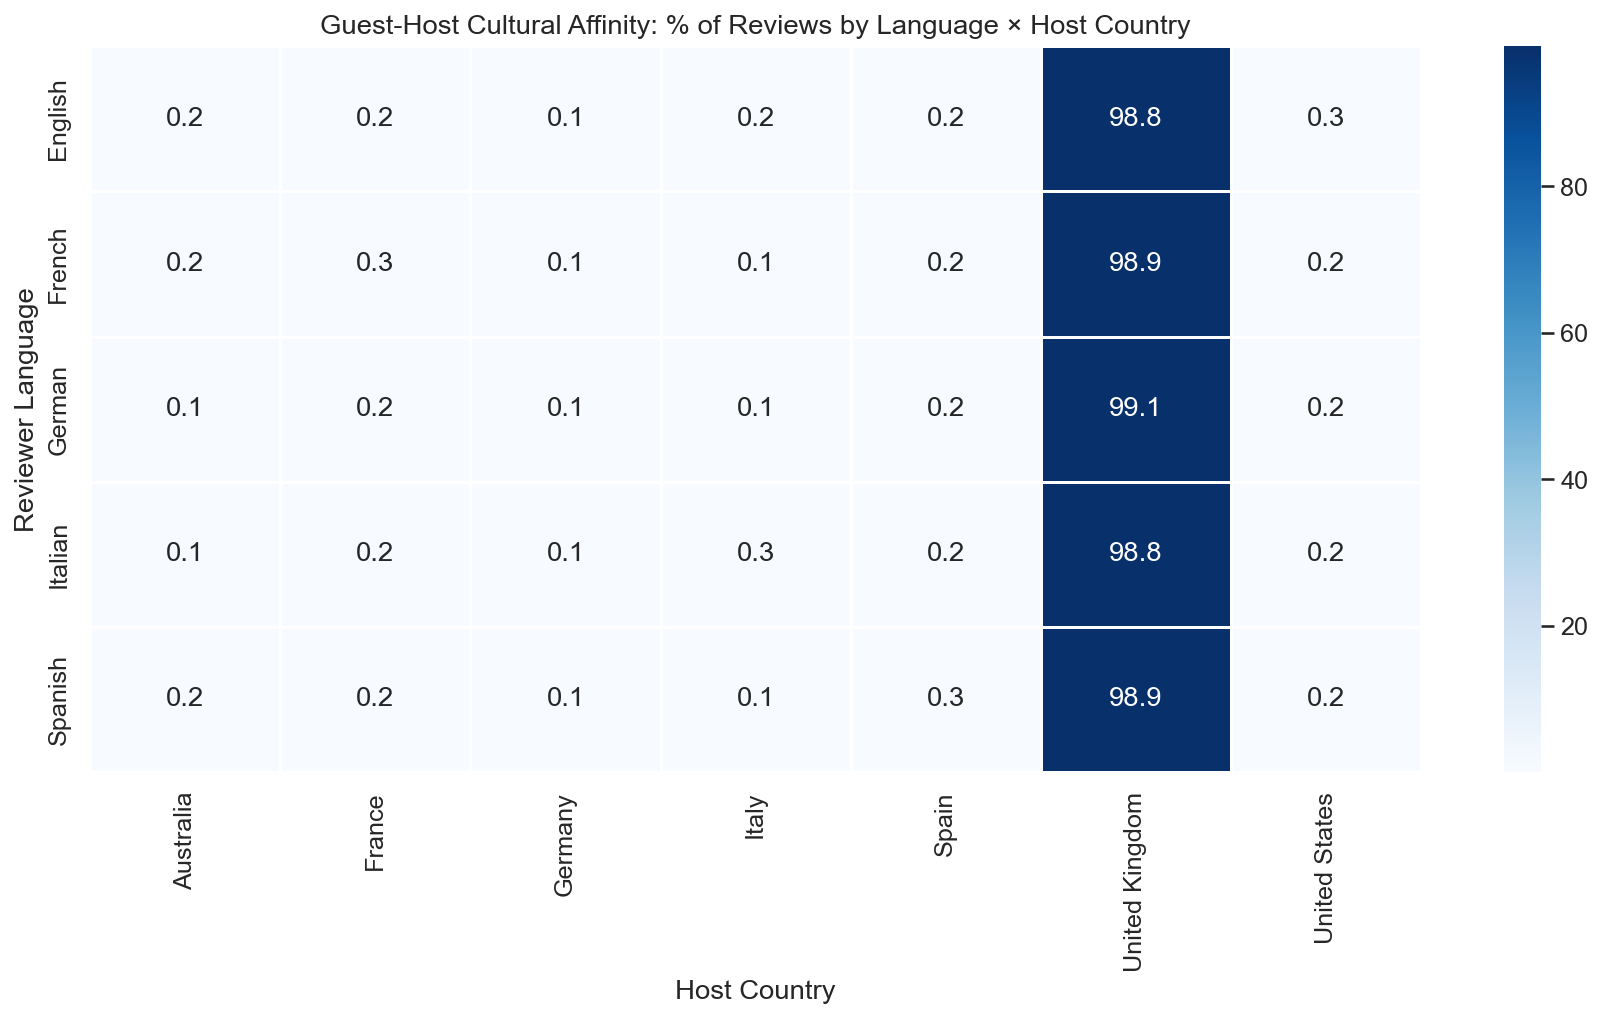
\includegraphics[width=0.65\textwidth]{cultural_affinity.png}
\caption{Guest--host cultural affinity matrix showing the percentage of reviews by reviewer language and host country. Some cultural clustering is visible but the pattern is dominated by UK hosts.}
\end{figure}

\subsection{Geographic Patterns}

Central London boroughs like \textbf{Southwark} (23.0\% non-English reviews), \textbf{Camden} (21.7\%), and \textbf{Westminster} (20.7\%) attract the most diverse international guests.
Outer boroughs like Sutton, Havering, and Bromley are almost exclusively reviewed in English.

A remarkable finding: \textbf{French is the most common non-English language in every single London borough} without exception.

\begin{figure}[H]
\centering
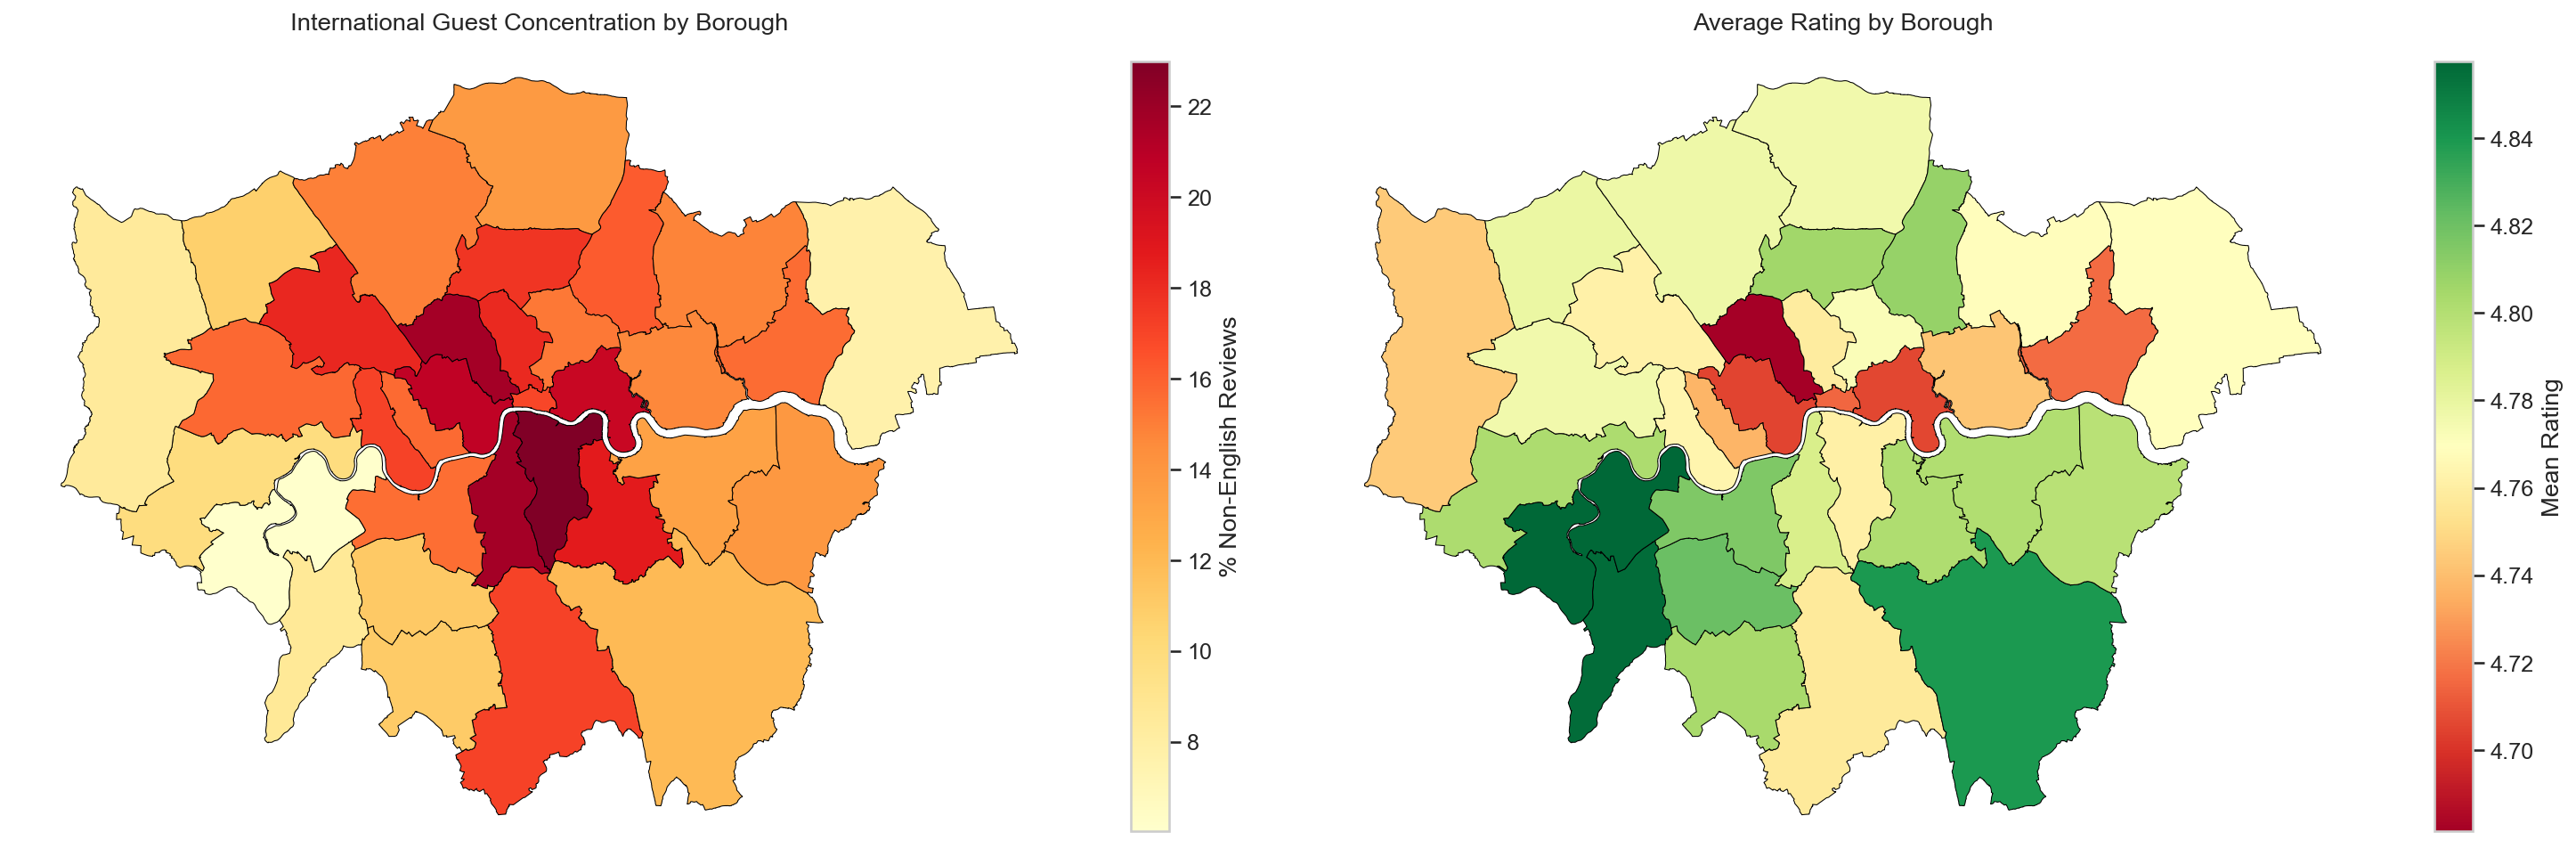
\includegraphics[width=0.9\textwidth]{borough_maps.png}
\caption{London borough maps. Left: percentage of non-English reviews (darker = more international). Right: average rating by borough.}
\end{figure}

\begin{figure}[H]
\centering
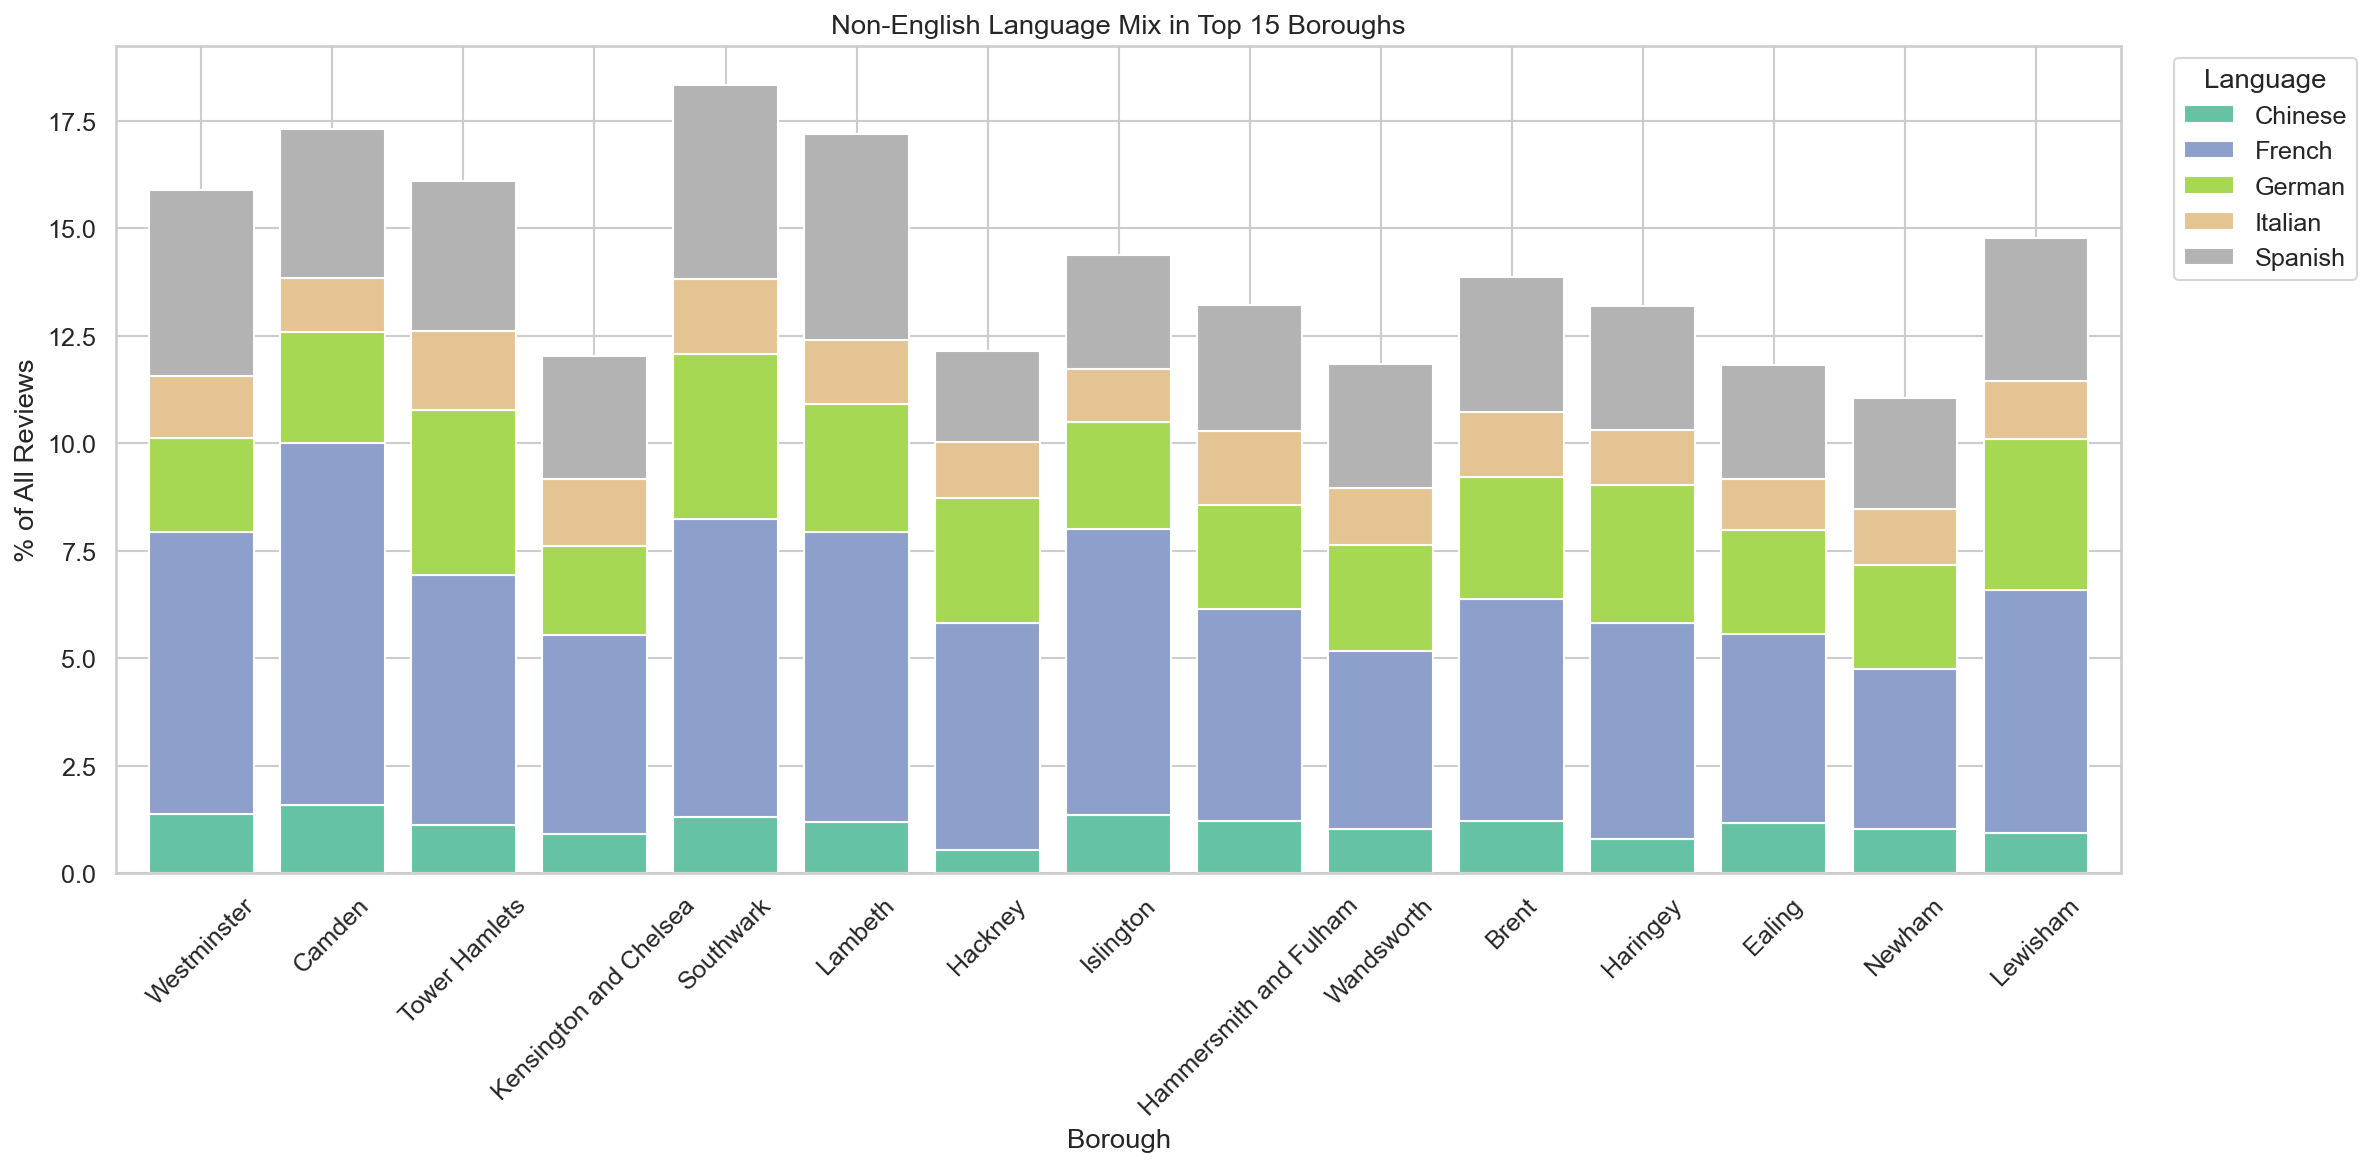
\includegraphics[width=0.85\textwidth]{borough_language_mix.png}
\caption{Non-English language composition in London's top 15 boroughs by review volume. French dominates everywhere.}
\end{figure}

\subsection{Review Length and Temporal Trends}

Cultural communication styles are also reflected in how much people write:

\begin{itemize}[nosep]
    \item \textbf{German} reviewers write the longest reviews (median 36 words).
    \item \textbf{French} and \textbf{English} reviewers write moderately (median 34 and 32 words).
    \item \textbf{Chinese} and \textbf{Japanese} reviewers write very short reviews (median 1 word), often just a brief comment or emoji.
    \item \textbf{Korean} reviewers fall in between (median 23 words).
\end{itemize}

\begin{figure}[H]
\centering
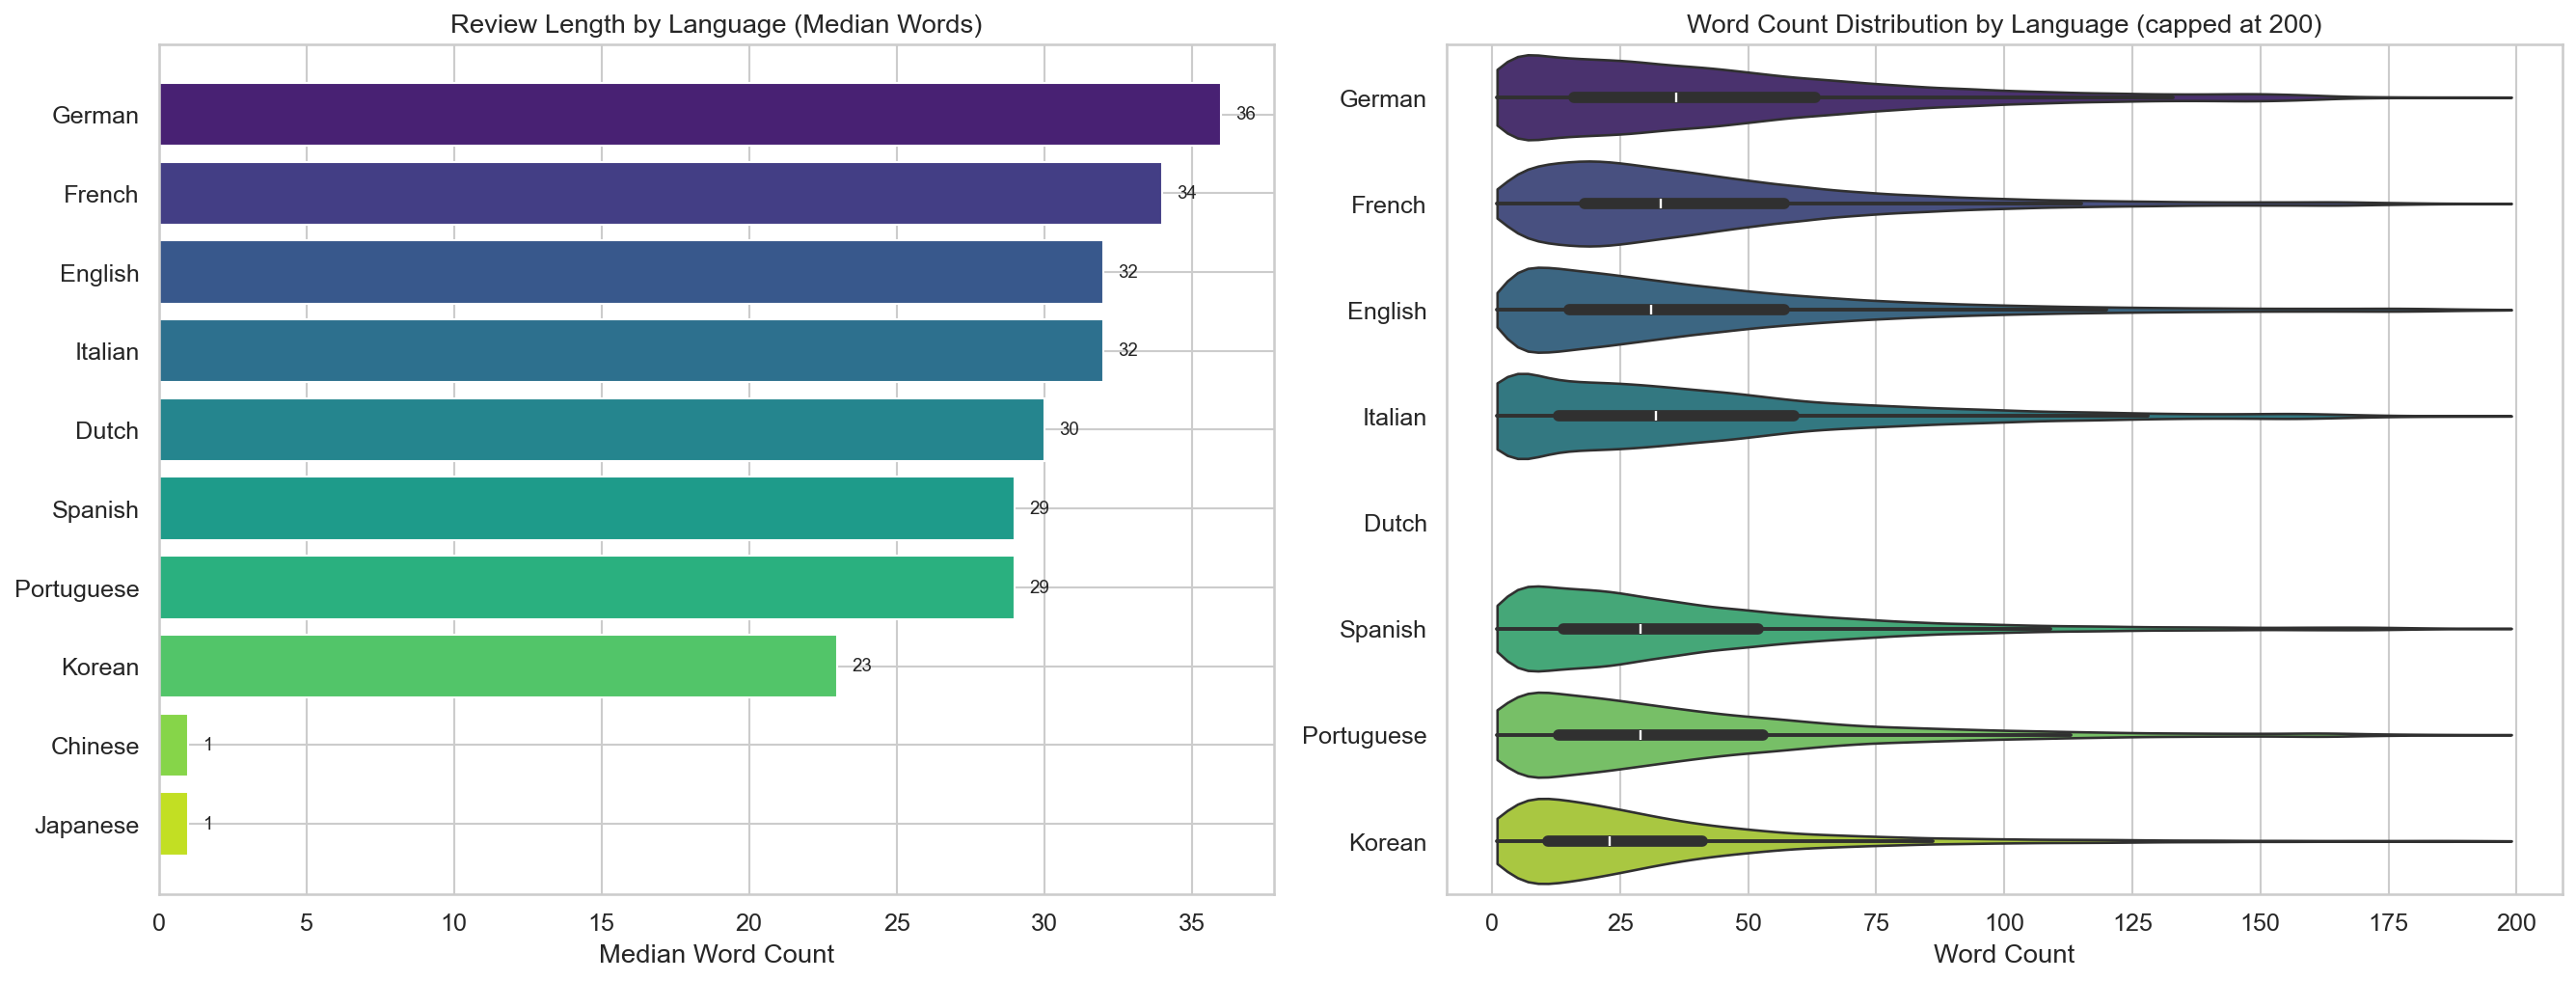
\includegraphics[width=0.85\textwidth]{review_length.png}
\caption{Review length by language. Left: median word count. Right: word count distribution (capped at 200 words). German reviewers are the most verbose; Chinese and Japanese the most concise.}
\end{figure}

The share of non-English reviews has grown significantly since 2015.
The seasonal heatmap reveals that French and Spanish tourists peak in summer (July--August), while Korean tourists are more evenly distributed.

\begin{figure}[H]
\centering
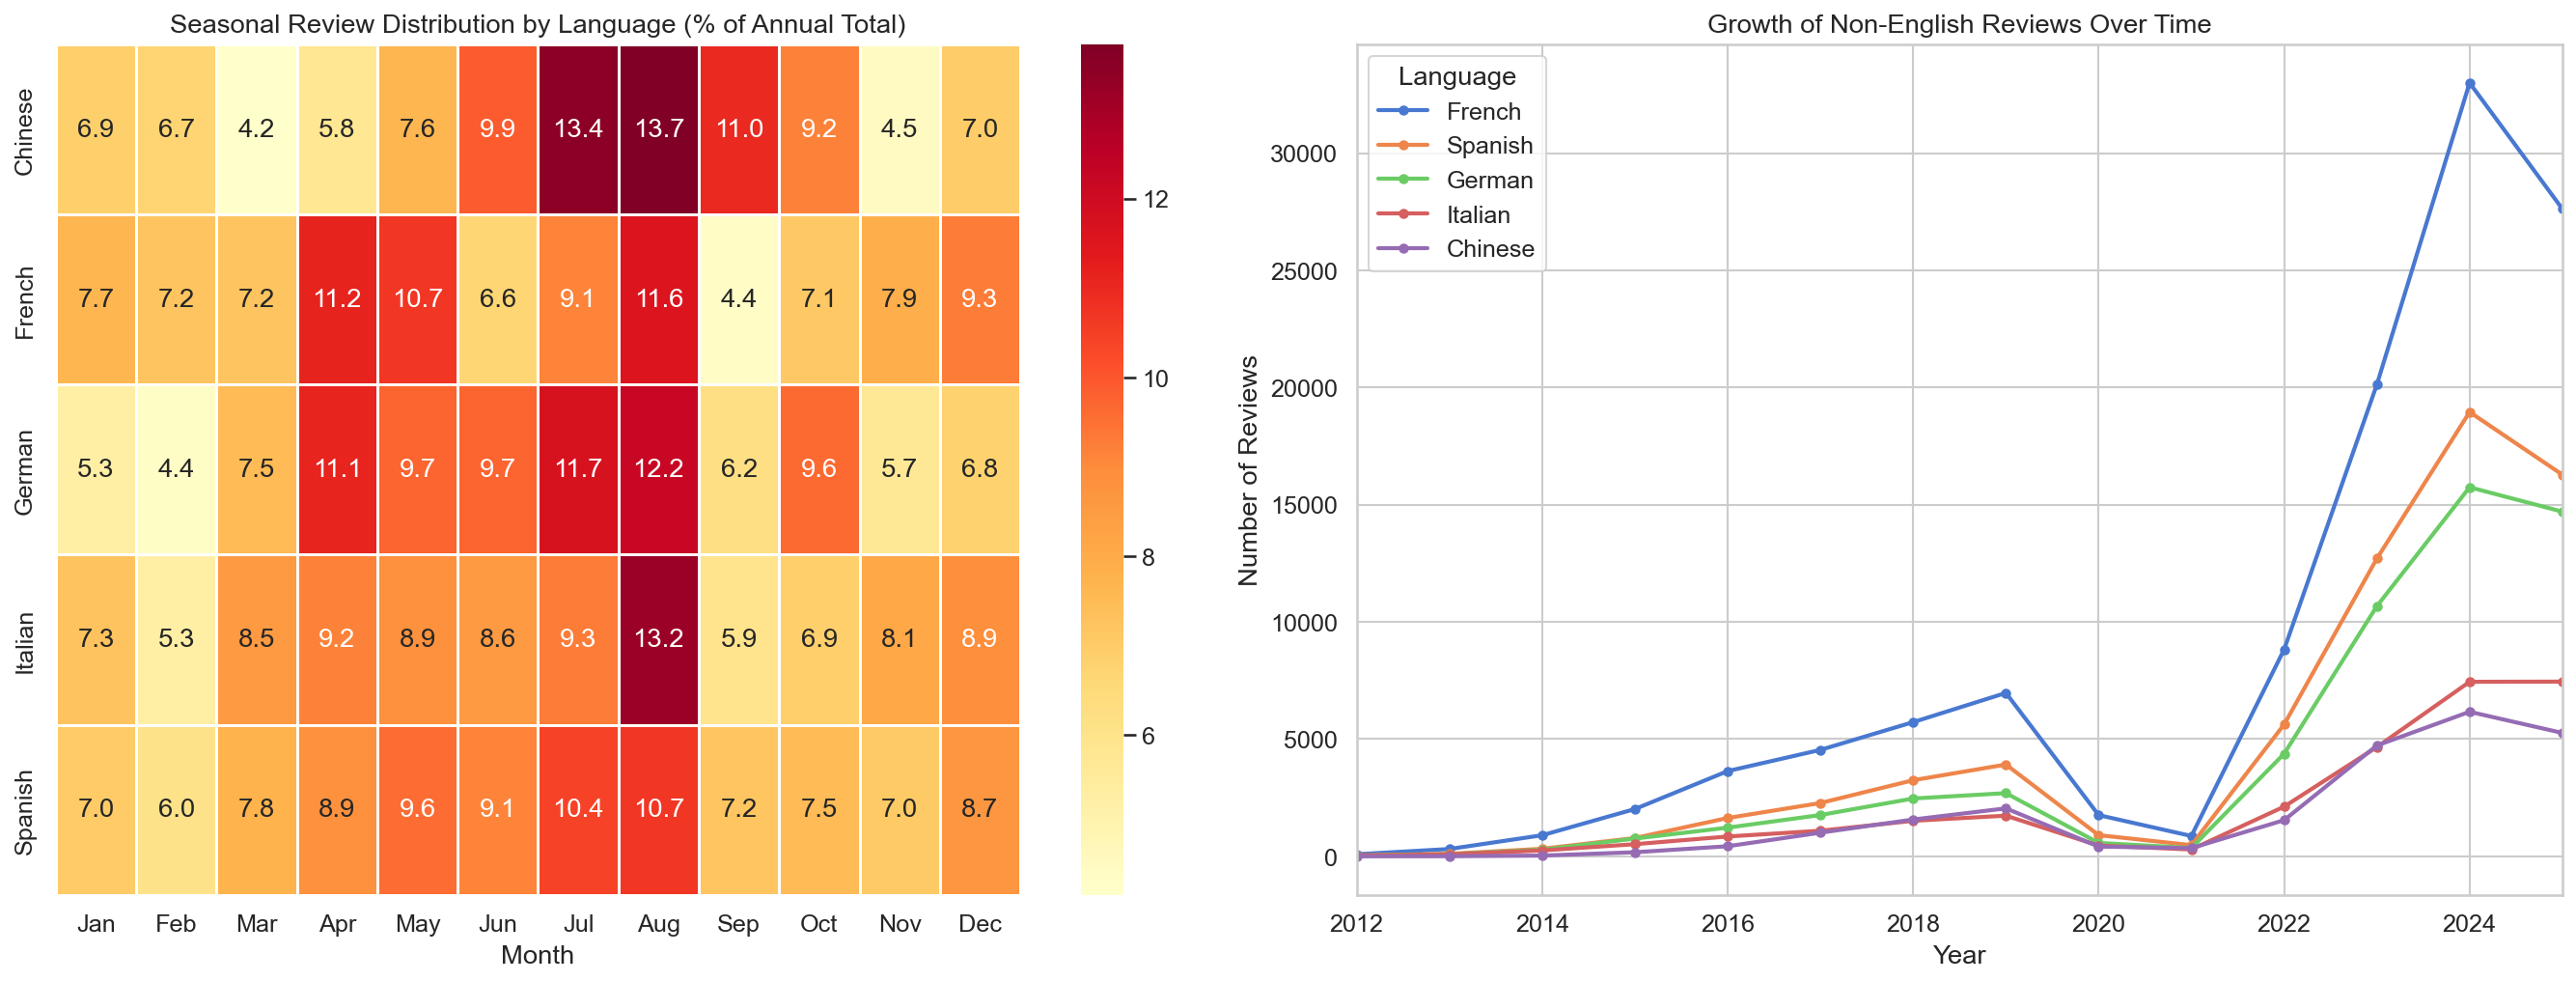
\includegraphics[width=0.85\textwidth]{temporal_trends.png}
\caption{Seasonal patterns (left heatmap) and long-term growth of non-English reviews (right). The internationalisation of London's Airbnb market accelerated after 2015.}
\end{figure}

% ============================================================
\section{Technical Setup}

All computation was performed on a single laptop:

\begin{table}[H]
\centering
\caption{Hardware and software environment}
\begin{tabular}{ll}
\toprule
\textbf{Component} & \textbf{Details} \\
\midrule
GPU         & NVIDIA GeForce RTX 3050 Laptop (4\,GB VRAM) \\
CUDA        & 12.4 (via PyTorch 2.6) \\
Python      & 3.11 (Miniconda) \\
NLP models  & VADER, Multilingual BERT, langid \\
Statistics  & scipy, scikit-posthocs \\
Geospatial  & GeoPandas, Folium \\
Key libraries & pandas, matplotlib, seaborn, transformers \\
\bottomrule
\end{tabular}
\end{table}

The GPU was used for multilingual BERT sentiment inference on 50,000 reviews.
The entire pipeline --- loading data, detecting 26 languages across 2.1 million reviews, running VADER sentiment, GPU BERT inference, aspect tagging, statistical tests, and generating all plots --- completes in approximately \textbf{43 minutes} on this hardware.

% ============================================================
\section{Limitations}

\begin{itemize}[nosep]
    \item \textbf{Language $\neq$ nationality.} A French-language review might come from Belgium, Switzerland, or Canada. Language is a cultural proxy, not a precise nationality indicator.
    \item \textbf{Rating compression.} Airbnb scores cluster heavily between 4.2 and 4.9. The absolute differences we found (0.05--0.09 points) are small even though they are statistically significant.
    \item \textbf{VADER is English-centric.} The VADER sentiment tool was designed for English text, which likely inflates the same-listing sentiment gap. We partially address this with the multilingual BERT model.
    \item \textbf{Listing-level scores.} The Airbnb dataset provides review scores at the listing level (aggregated), not per individual review, which limits per-review precision.
    \item \textbf{Selection bias.} Guests who write reviews are not representative of all guests. Review-writing propensity may itself vary across cultures.
    \item \textbf{Language detection accuracy.} While langid is generally reliable ($\sim$95\% accuracy for major languages), it can misclassify very short or multilingual reviews.
\end{itemize}

% ============================================================
\section{Conclusion}

We built a complete pipeline that reads 2.1 million Airbnb reviews from London, identifies 26 languages, and shows that \textbf{culture significantly shapes how guests rate their stays}.

The key findings are:
\begin{enumerate}[nosep]
    \item \textbf{Ratings differ by language.} Korean speakers rate highest ($M = 4.773$); Spanish speakers rate lowest ($M = 4.679$). All seven rating dimensions show significant differences (Kruskal-Wallis $H > 10{,}000$, $p < .001$).
    \item \textbf{The gap persists on the same listing.} English reviews are more positive than French, German, Spanish, Italian, Dutch, and Portuguese reviews on \emph{identical properties} (Cohen's $d > 3.0$, $p < .001$).
    \item \textbf{Cultures emphasise different aspects.} Communication and location have the strongest cultural variation (Cram\'{e}r's $V = 0.28$ and $0.24$). Price concerns are relatively universal ($V = 0.05$).
    \item \textbf{French dominates internationally.} French is the top non-English language in all 33 London boroughs, accounting for 5.6\% of all reviews.
    \item \textbf{Writing styles differ dramatically.} Germans write 36-word reviews; Chinese and Japanese reviewers write 1-word reviews.
\end{enumerate}

The practical implication is clear: \textbf{a star rating is not culturally neutral}.
A host with many French or Spanish guests may have a lower average score than a host with mainly Korean guests, even if both provide identical service.
Airbnb could consider developing culturally-aware review summaries or normalising ratings by reviewer background to create a fairer system.

Future work could extend this analysis to other cities (Paris, Barcelona, Tokyo), incorporate cultural dimension frameworks like Hofstede's indices, and develop culturally-adjusted rating models.

\end{document}
